%Preamble
\input{setup/preamble.tex}% package inclusion 
\usepackage{dirtytalk}
\usepackage{svg}
\usepackage{amsmath}
\usepackage{xcolor}

\usepackage{afterpage}

\newcommand\blankpage{%
   \null
   \thispagestyle{empty}%
   \addtocounter{page}{-1}%
   \newpage}
%and set up of the document
\input{setup/hyphenations.tex}% 
\input{setup/macros.tex}% my new macros

%Tikz for flowcharts:
\usepackage{tikz}
\usetikzlibrary{shapes.geometric, arrows}

%Start/stop ellipse:
\tikzstyle{startstop} = [ellipse, minimum width=3.2cm, minimum height=1cm, text centered, text width=2.2cm, draw=black, fill=blue!30]

%\tikzstyle{startstop} = [rectangle, rounded corners, minimum width=2cm, minimum height=1cm,text centered, text width=3cm, draw=black, fill=red!30] 

%Out trapezium:
\tikzstyle{io} = [trapezium, trapezium left angle=70, trapezium right angle=110, minimum width=1cm, minimum height=1cm, text centered, text width=2.2cm, draw=black, fill=blue!30]

%Process rectangle:
\tikzstyle{process} = [rectangle, minimum width=6.2cm, minimum height=1cm, text centered, text width=5.2cm, draw=black, fill=orange!30]

%Decision diamond:
\tikzstyle{decision} = [diamond, minimum width=2cm, minimum height=1cm, text centered, text width=2.5cm, draw=black, fill=green!30]

%Arrows:
\tikzstyle{arrow} = [thick,->,>=stealth]

%Guidebox rectangle:
\tikzstyle{Guidebox} = [rectangle, minimum width=0cm, minimum height=0cm]

%Caption rectangle:
\tikzstyle{Caption} = [rectangle, minimum width=0cm, minimum height=0cm, text centered, text width=14.5cm]

%Black dots:
\tikzstyle{Blackdot} = [circle, minimum width=0.6cm, minimum height=0.6cm, text centered, text width=0.1cm, draw=black, fill=black!200]

%Main Document
\begin{document}
    %The preface and title
    \pagestyle{empty}
    \pagenumbering{roman}
    \pdfbookmark[0]{Front page}{label:frontpage}
\begin{titlepage}
    \addtolength{\hoffset}{0.5\evensidemargin-0.5\oddsidemargin}
    \noindent%
    \begin{tabular}{@{}p{\textwidth}@{}}
        \toprule[2pt]
        \midrule
        \vspace{0.2cm}
        \begin{center}
            \Huge{\textbf{
                BB-1
            }}
        \end{center}
        \begin{center}
            \LARGE{
                Bilka Bot-1
            }
        \end{center}
        \begin{center}
            \Large{
                A guidance robot
            }
        \end{center}
        
        \vspace{0.2cm}\\
        \midrule
        \toprule[2pt]
    \end{tabular}
    %a better picture for cover would be nice, maybe a figure of the robot itself
    \begin{figure}[H]
        \centering
        \includegraphics[width=0.75\textwidth]{figures/aau_logo_en.pdf}
        %\caption{}
        \label{fig:Frontpage}
    \end{figure}
    \vspace{1 cm}
    \begin{center}
        \large{
            ROB 5 
        }
        \\
        \vspace{0.2cm}
        \Large{
            19Gr566
        }
    \end{center}
    \vfill
    \begin{center}
        Robotics\\Aalborg University
    \end{center}
\end{titlepage}
    \pdfbookmark[0]{English title page}{label:titlepage}
\aautitlepage{%
    \englishprojectinfo{
        %title
        BB-1
    }{%
        %theme
        Social Robots 
    }{%
        %project period
         Autumn 2019
    }{%
        %project group
        ROB 566
    }{%
        %list of group members
        Ibrahim Jad Masri\\
        Jonathan E. Schmidt\\
        Kristian Daugaard\\
        Mark R. Blankensteiner\\
        Natalie Mark\\
        Valdemar J. Qvist
        
        
  }{%
        %list of supervisors
        Karl Damkjær Hansen
        
  }{%
        % number of printed copies
        1 
  }{%
        % date of completion
        \today 
  }%
}{%
    %department and address
    \textbf{Robotics}\\
    Aalborg University\\
    Department of Electronic Systems\\
    Fredrik Bajers Vej 7B\\
    DK-9220 Aalborg

    \href{http://www.robotics.aau.dk}{http://www.robotics.aau.dk}
}{% the abstract
}
    \chapter*{Preface}\label{ch:prefacev}

\vspace{\baselineskip}\hfill Group {566}, Aalborg University, \today
\vfill\noindent


\begin{minipage}[b]{0.45\textwidth}
    \centering
    \rule{\textwidth}{0.5pt}\\
    Ibrahim Jad Masri\\
    {\footnotesize <ijadma17@student.aau.dk>}
\end{minipage}
\hfill
\vspace{3\baselineskip}
\begin{minipage}[b]{0.45\textwidth}
    \centering
    \rule{\textwidth}{0.5pt}\\
    Jonathan Eichild Schmidt\\
    {\footnotesize <jschmi17@student.aau.dk>}
\end{minipage}

\begin{minipage}[b]{0.45\textwidth}
    \centering
    \rule{\textwidth}{0.5pt}\\
     Kristian Daugaard\\
    {\footnotesize <kdauga17@student.aau.dk>}
\end{minipage}
\hfill
    \vspace{3\baselineskip}
    \begin{minipage}[b]{0.45\textwidth}
        \centering
        \rule{\textwidth}{0.5pt}\\
       Mark Richard Blankensteiner\\
        {\footnotesize <mblank16@student.aau.dk >}
    \end{minipage}

\begin{minipage}[b]{0.45\textwidth}
    \centering
    \rule{\textwidth}{0.5pt}\\
     Natalie Mark\\
    {\footnotesize <nmark15@student.aau.dk>}
\end{minipage}
\hfill
    \vspace{3\baselineskip}
    \begin{minipage}[b]{0.45\textwidth}
    \centering
    \rule{\textwidth}{0.5pt}\\
    Valdemar Jul Qvist\\
    {\footnotesize <vqvist17@student.aau.dk >}
 \end{minipage}
    \chapter*{Acronyms and abbreviations}\label{ch:acronyms}

\begin{table}[H]
\begin{tabular}{ll}
\textbf{Acronym} & \textbf{Definition} \\
HRI & Human Robot Interaction \\
ISO & International Organization for Standardization\\
DSZ & Dynamic Social Zone\\
RGB-D & Red, Green, Blue \& Depth\\
IR & Infra-Red\\
FOV & Field Of View  \\
LIDAR & Light Detection and Ranging\\
TOF & Time Of Flight\\
HDDM & High Definition Distance Measurement\\
GUI & Graphical User Interface\\
ROS & Robot Operating System\\
BLOB & Binary Large Objecs\\
PDF & Probability density function
\end{tabular}
\end{table}
    \pdfbookmark[0]{Table of Contents}{label:contents}
    \titlespacing{\chapter}{0.5cm}{1cm}{0.5cm}
    \setlength\parindent{0em}
    \begingroup
        \let\cleardoublepage\clearpage %for removing the empty page before ToC
        \tableofcontents
    \endgroup
    \clearpage
    
    %Main part of text
    \pagestyle{fancy}
    \pagenumbering{arabic}
    
    %Input of Problem Analysis
    \part{Problem analysis}\label{Part:PA}
\chapter{Introduction}\label{ch:introduction}
Many traditional daily activities, like grocery shopping or home depot shopping, have entered the world of e-commerce. A large number of companies offer services that will bring you, your self-chosen groceries straight to your door step. This may seem like an improvement of the old-fashioned way of going to a store. However, one of the issues with online grocery shopping, is the ability to see, feel and smell the goods, and this goes for especially the fresh items like fruits and vegetables \cite{GroceryDive}.\\

Customers are steadily getting accustomed to the idea of purchasing online, and not only non-foods. This means that the stores have been converting more of their sales from the physical stores to the online version for the past couple of years \cite{Quartz}. This could indicate that customers may be ready to let go of the traditional shopping method in exchange for extra time on their hands.\\
\\
Shopping online offers the possibility for knowing whether an item is available or not as well as makes finding the items in the store easier whereas this is not as effortless when going to physical store. This is due to it requiring time and energy and asking for help may not always be as easy as it may sound. F.Lee (2002) \cite{AskingHelp} discusses three problematic aspects of asking other people for help. The first is accepting lack of competence to complete a task. By asking for help, you acknowledge that you can not finish a task, either in time or at all by yourself. Secondly, it involves accepting inferiority to other people. By asking them, you agree that you think they may be better equipped to complete this task than yourself. Lastly, it involves accepting a level of dependency of other people. A robot helper might not entirely remove these factors, as the person would still have to accept these things, but removing the human interaction might alleviate some of the pressure and encourage customers to ask the robot for help.\\

Pros and cons being presented for both online and traditional shopping, a middle way could be a way of utilising the pros of each method for shopping. A new method could be introduced that would reduce the time spent shopping compared to the traditional way. This method would still allow self inspection of wares and lowering or removing the anxiety related to asking employees for help, while lowering the running costs of a store, by lowering the amount of employees needed for costumer service.

\newpage
The case for this will be presented as follows:\\

\textit{A robot that can guide customers around in hypermarkets (e.g. Bilka, Silvan, Target, Walmart) to reduce time spent searching for items and reduces/eliminates the need for employees to be present for customers in need of assistance with locating wares. This means that the running costs of the store could potentially be lowered and the time consumption is reduced for the customers, while still giving the customers the choice to choose their goods from the shelves. This can be coupled with the company's online shop, to allow for a pre-built shopping list with immediate guidance upon arrival or the robot can offer a look at the stores full selection of items via a monitor. The robot is meant to be part of a fleet that would operate in collaboration with each other in the warehouse, as a store will typically have more than one customer at a time.}\\

Designing a robot as described above requires many problems solved. This includes: navigation, path planning, interaction with surroundings and social interaction.\\

\textbf{Navigation} is a crucial part of a solution that revolves around guiding people to specific locations. If the robot cannot locate itself, it cannot complete a given task. Navigating around a store includes mapping both static and dynamic objects.\\

\textbf{Path planning} is a part of navigation, in the sense that it is also important to deal with the robots decision making program, as not all paths may be equally time efficient. This will also be the part of the navigation that deals with dynamic objects and obstacles.\\

\textbf{Interaction with surroundings} revolves around the use of sensors to give the robot the ability to react to its surroundings. This can include pictures/video, range tracker and software to translate the sensor data into data that can be processed and yield information about proximity of objects, whether they are moving or not (depending on the frequency of the system).\\

\textbf{Social interaction} is inevitably a part of designing a robot that is intended to operate within the same boundaries as humans. This will include giving the user a good experience based on the robots behaviour. It is important for humans to feel safe and comfortable around the robot for the best customer experience, including best management of time spent at the store.\\

    \chapter{Previous Solutions}\label{ch:PrevSol}
To understand the concept of social robots and how they work with and around humans it can be beneficial to look into how these robots have previously been implemented. Looking at these robotic proposals can help highlight some of the necessities as well as common issues when implementing a social robot. The findings from these projects will be a starting point of research for this project to develop a social robot for assisting humans in a hypermarket.

\section{Care-O-Bot}\label{sec:cob4}
Care-O-Bot, as seen in figure \ref{fig:cob4}, is developed at Fraunhofer Institute for Manufacturing Engineering and Automation in Germany. It is a mobile robot that is used to assist humans in semi-structured environments. It is built to be used in research areas and to support people in their daily life in a variety of situations. The development of Care-O-Bot began in 1998 and version 4 was released in 2015 \cite{cob4}.

\begin{figure}[H]
    \centering
    \begin{minipage}[b]{0.52\linewidth}
        Care-O-Bot 4 is designed to be configured for specific situations, where an arm or two can be attached to it. The modularity extends to having spherical joints in the neck and hips which allows for 360 degrees of rotation in head and torso, respectively. The design of the robot was based on social role models in order to be accepted socially and interact with humans. This was done by considering three levels of human emotional reaction to everyday use when building the robot. These three levels are visceral, behavioural, and reflective which include appearance, pleasure and effectiveness of use as well as self-image, personal satisfaction and memories \cite{cob4}.
    \end{minipage}
    \hspace{0.42cm}
    \begin{minipage}[b]{0.43\linewidth}
        \centering
        \includegraphics[width=\textwidth]{figures/Cob4.jpg}
        \caption{Care-O-Bot 4 developed by Fraunhofer \cite{cob4_image}.}
        \label{fig:cob4}
    \end{minipage}
\end{figure}

Care-O-Bot 4 is designed to have human features such as posture and natural arm movements. For example, the robot leans forward as a way of showing respect while staying balanced and keeping eye contact. Facial expression, represented by a a pair of eyes, are shown on a touch screen embodied on the robot’s head to express emotions and social cues. The screen is also used to interact with the robot when a user approaches it by showing a graphical user interface. By using the hip and neck joints, the screen can be positioned according to the user's direction \cite{cob4}.

The robot has a microphone that is used to recognise speech, in addition to cameras for recognising persons and hand gestures. Care-O-Bot has speakers and multiple LEDs to indicate the inner state of the robot and a laser pointer to show which object the robot is about to grasp. It is also equipped with 3 laser scanners to avoid obstacles and 3D-RGBD camera in the gripper in order to determine the position of objects \cite{cob4}.


\section{SPENCER}\label{sec:spencer}
SPENCER is a robot assistant, with the purpose of informing and guiding passengers in airports. One of the specific tasks is to bring passengers, travelling with connecting flights, from their arrival gate to the passport control. SPENCER learns human social behaviour to plan appropriate actions in real-time\cite{SPENCER_paper}.
%photo

\begin{figure}[H]
    \centering
    \begin{minipage}[b]{0.485\linewidth}
        SPENCER is designed with a human-inspired abstract appearance, as seen figure \ref{fig:SPENCER_design}. It should look human-like to not appear as unfriendly or threatening, which is an important factor when a robot is interacting with humans, but also not too much like a human, which can lead to disappointment or refusal of the system. This concept is elaborated in section \ref{sec:Psychology}.
        As seen on figure \ref{fig:SPENCER_design}, the robot has a round head with two eyes and mouth in the shape of a smile, making it appear friendly.
        To physically interact with the user, the robot has a touchscreen and a scanner for boarding pass. The sensors in SPENCER consists of two SICK LMS 500 2D laser scanners, multiple RGB-D cameras and a stereo camera system.
    \end{minipage}
    \hspace{0.2cm}
    \begin{minipage}[b]{0.48\linewidth}
        \centering
        \includegraphics[width=\textwidth]{figures/SPENCERpic.png}
        \caption{Design view and actual appearance of SPENCER robot\cite{SPENCER_paper}. An EU funded research project, tested for KLM in Amsterdam Schiphol airport to manage the passengers flow \cite{SPENCERCITE}. }
        \label{fig:SPENCER_design}
    \end{minipage}
\end{figure}

As a middle-ware for the software components, ROS is used\cite{SPENCER_paper}.
The data from the 2D laser data is used for detecting people. The robot will detect people and divide them into multiple groups. After forming groups, the robot can determine what group of people is interacting with it and who is in need of guidance. %They compute features for segments from the data and classified.
As long as one member is following SPENCER, it is considering the group as following.\\

The robot is using algorithms for both mapping the environment and calculating the probability of the direction of dynamic objects, which is used to predict the direction of moving objects. When planning the route, it is needed to take the social rules into consideration. The robot should not cross through another group of people, but deviate it, when moving to the destination. This is why SPENCER uses a human-aware cost map that makes a path around the group of people detected and SPENCER also moves in a path avoiding abrupt motions by anticipating future collisions and adapting the velocity accordingly\cite{SPENCER_paper}.


\section{Intelligent Shopping Trolley}\label{sec:IST}
The Intelligent Shopping Trolley (IST) is an intelligent system to notify costumers of deals and scheduling the shortest obstacle-free path for the user.
The paper \ref{fig:trolleyRep} states that the real-time communication with the costumer helps with detection of preferences and gives feedback, which can assist them in their daily shopping. Where the real-time communication is a setup of the sensors applied on the trolley to monitor the users behaviour, such as stopping or walking by a specific product. This data is then sent back to the retailer so that they can spectate the results of the costumers using the trolleys and have a real-time communication with them.\\

The solution is run through a system where routers has been set up in each product shelf of the hypermarket, as seen in figure  \ref{fig:trolley2}. Whenever the person passes a sale the trolley will alert the user about the current sales that he or she is passing. The IST also directs the user to the desired products that they need and the conclusion is that the IST users benefit from non-time consumption when using the routes laid out for them.\\
\\
Two pressure sensors, which can be seen on figure \ref{fig:trolley1}, is used to determine whether the trolley is being used or not. The grip of a person exerts a pressure that results in increase in voltage and hereby it can be detected. If the customer leaves the trolley for more than 30 minutes, the trolley is treated as unused and the server will notify an employee to retrieve that trolley.
A G-sensor is used to determine the acceleration of the trolley, and to determine the aforementioned, if the user is stopping at certain wares. The trolley is connected with a module, that wireless connects the trolley with the routers.\\
The overall idea of how the IST system works can be seen on figure \ref{fig:trolleyRep}.

\begin{figure}[H]
    \begin{minipage}[b]{0.5\linewidth}
        \centering
        \includegraphics[width=\textwidth]{figures/ISTTrolley.png}
        \caption{The IST system showing where the pressure sensor and the control box is placed\cite{wangintelligent}}
        \label{fig:trolley1}
    \end{minipage}
    \begin{minipage}[b]{0.5\linewidth}
        \centering
        \includegraphics[width=\textwidth]{figures/ISTTrolley2.png}
        \caption{The IST system showing where the wireless router is placed on a product shelf\cite{wangintelligent}}
        \label{fig:trolley2}
    \end{minipage}
\end{figure}

The interaction between the user and the trolley happens through an LCD touch panel in the control box as seen in figure \ref{fig:trolley1}. The customer can search for the location of specific products, and as a result, the shortest obstacle-free path will be provided for the customer. In addition, information such as promotions and products on sale is also shown on the LCD screen.\cite{wangintelligent}.

\begin{figure}[H]
    \centering
    \includegraphics[width=0.75\textwidth]{figures/trolley.png}
    \centering{\caption{A representation of an intelligent trolley \cite{wangintelligent}}\label{fig:trolleyRep}}
\end{figure}

%The path-planning consists of a modified A* algorithm.
The servers can determine where all of the trolleys are positioned, which is used when planning a route to a desired product, so a customer would not collide with another trolley. The server can also analyse and record the customer's behaviour in the retailer's database. This data can be used for determining product shelves that have been visited more often, finding the potentially popular products \cite{wangintelligent}.
\\
\\
%End of chapter
These solutions highlight the current approaches to social robots in environments with multiple humans. The findings from these show that it is important to create a robot that can navigate between humans while insuring that it is safe and comfortable for the humans.
    
    \chapter{Human-Robot Interaction}\label{ch:HRI}
Interaction between humans and robots play an important role when developing robots that are meant to operate in environments shared with humans. They should take safety, dynamic surroundings and social aspects into consideration when making decisions.

\section{Metrics for measuring the performance of HRI}
The success of human-robot interaction can be difficult to quantify. The metrics for measuring this, will be relevant when evaluating the solution towards the end of the report, to have quantifiable results to discuss. This section will not disclose on topics like execution speed, since this is an already quantified metric, but will deal with the abstract but still important aspects, like social encounters. A paper by Carnegie Mellon University \cite{HRIMetrics} examines aspects like trust, user engagement and compliance, and how these affect the interaction. Since the robot is supposed to function on its own, it needs to be equipped to deal with various situations.
\subsection{Interaction Characteristics}
Analysing how robots can interact with humans can be a great tool to improve the experience for the users. This could be done by, e.g. observing the style of interaction. In the case of a robot that guides people to locations, this could be done with a GUI mounted on the robot itself. This would create little to no interaction, as the robot serves a purpose different than interaction, making it less relevant for this project than e.g. a robot whose sole purpose is interaction.
\subsection{Trust}
Trust is likely to influence the result of a human-robot interaction. Humans will react differently to different situations and unforeseen situations occur. This may affect the trust of the robot, and this will as a result change the behaviour towards the robot. For example, if a guidance robot were to make a mistake, say an obstacle made the path longer than intended, it is important that the human trusts the robot with the next decision. If not, the human might walk away and the interaction is a failure.
\subsection{Engagement}\label{subsec:Engagement}
It is important to engage with a user to capture attention. This can be accomplished by using social characteristics of interactions like emotions and dialogue. If a user has no interest in a robot, there will not be given any attention and the interaction might not even happen at all. This might be less relevant in the case of a guidance robot, as the robot serves a specific purpose and by this, the robot might not need to capture the users attention alone based on engagement, as the users would typically need some assistance from the robot \cite{HRIMetrics}.
\subsection{Compliance}
Cooperation from humans is relevant when discussing human-robot interactions. Appearance and norms expected by humans, might influence how cooperative a user will be. A theoretical example could be, that if a robot looked like something humans usually dislike, such as something scary or just uneasy, they might refrain from using the robot entirely. If the robot is loud and disturbing, they might also feel a desire to not participate. As mentioned in the subsection \textbf{engagement}, other fields of robotics might benefit more from this topic such as health care, although it might still prove useful when designing and implementing the solution \cite{HRIMetrics}.

\section{Psychology}\label{sec:Psychology}
A paper on human psychology and interaction with robots, called “Human-robot proxemics: physical and
psychological distancing in human-robot interaction”\cite{mumm2011human}, was written by J. Mumm and B. Mutlu, describing the demands for appropriate behaviour when integrating robots into a human environment.
Interacting with humans can seem like a small feat, however behaviour such as inappropriate distancing and continuous eye contact can result in humans distancing themselves to the particular robot.\\

A key factor to estimate before sending a robot out in a social environment is \textit{proxemics} - the study of personal space. The different cues humans make when another person or robot is disruptive of this space can be captured by sensors and cameras and it is essential to keep in mind when designing a robot to work in healthcare \cite{mumm2011human}.\\
When studying proxemics the author of the interpersonal distancing needs to be mentioned - Edward T. Hall designed a measurable chart of zones. These zones can be described as such:\\
\begin{itemize}
    \item intimate zone
    \item personal zone
    \item social zone
    \item public zone
\end{itemize}
With these 4 zones an estimation of where the robot should be placed to avoid the discomfort of entering a intimate zone can be measured. See figure \ref{fig:hall} for precise measurements of where the zone starts and begins.

\begin{figure}[H]
    \centering
    \includegraphics[width=0.75\textwidth]{figures/hall.png}
   \caption{The 4 different zones/phases of a distancing chart made by Edward t. Hall, to measure different comfort zones \cite{Hall}}
    \label{fig:hall}
\end{figure}

The personal space has been heard of before as a intimate space belonging to the person inside that zone, this is psychologically considered theirs. Entering this space is considered intimate and is not desired from a robot used to guide people around. However, it would be likeable to minimum enter the social zone. This zone is where it is described as likeable to enter a conversation with another person due to the safe distancing to the person and normally when following a person this zone would be optimal as well. And the public zone is a zone where people will most likely ignore the fact that the robot is trying to communicate with them, so to conclude - with Hall's model of interpersonal spacing the most desirable comfort zone the robot should operate in is the social zone, which is described as 1.2m as the "close-zone". Small deviations into the public zone will likely occur when the person guided is following the robot \cite{Hall}.\\

Another model is the \textit{Compensation model} this is not defined by space, like Hall's model, but rather suggesting non-verbal equilibrium between two persons. This means that when e.g. person A increase closeness in form of keeping eye contact, then the likeable other, person B, should compensate for this increase by decreasing the closeness by averting his/her gaze, or physically distancing themselves to person A. This can be used as a guideline for human-robot interaction so that sensors alert the system when noticing some of these cues.\\
Elaborating on the research in the paper this project deduced that a model was derived from the research on nonverbal cues, that described that the person will have to distance themselves to the robot, if the robot kept maintaining eye contact. Another model is proposed called the \textit{attraction-transformation model}, to connect the verbal and nonverbal cues,to avoid people disliking the robot due to disruption of the personal space.\\
\\
A resemblance can be seen between non-verbal contact and likeness of the robot. If the person has prejudices about a certain robot, averting its eyes can be a good response, because then the person will not feel as if they interact with it on a personal level. A way to avoid this is to either follow these guidelines or design a robot that has no close relation to a human being, because a human wont perceive a metal arm the same way as they perceive a human-like robot. However, it is important to have a robot with close human resemblance (but not too much) for the user to feel more secure \cite{mumm2011human}, e.g. \textit{Telenoid}, as seen in figure \ref{fig:telenoid} and figure \ref{fig:telenoid2}.

\begin{figure}[H]
    \begin{minipage}[b]{0.36\linewidth}
        \centering
    \includegraphics[width=\textwidth]{figures/telenoid.jpeg}
    \caption{A social robot, Telenoid R1 by Hiroshi Ishiguro\cite{telenoidIMG}.}
    \label{fig:telenoid}
    \end{minipage}
        \hspace{0.2cm}
    \begin{minipage}[b]{0.60\linewidth}
        \centering
        \includegraphics[width=\textwidth]{figures/telenoid2.jpeg}
        \caption{A man holding and interacting with the Telenoid robot\cite{telenoidIMG}.}
        \label{fig:telenoid2}
    \end{minipage}
\end{figure}

The uncanny valley illustration describes the aforementioned statement, that the likeness of a human being can be advised against, as seen in figure \ref{fig:uncanny}.

\begin{figure}[H]
    \centering
    \includegraphics[width=.75\textwidth]{figures/uncannyvalley.png}
    \caption{Uncanny valley graph, is a model, that describe the humans reaction to an industrial robot manipulator, a robot like wall-E, almost human like to a perfect human robot. If the robot falls into almost human-like it falls into the uncanny valley, it looks like a person, but the movement might be putting people off because of the resemblance to a walking dead 
    \cite{mori2012uncanny}.}
    \label{fig:uncanny}
\end{figure}

It can be seen that when closing in on 100\% human likeness the affinity drops to a negative effect and people starts feeling it is wrong. 
Presenting movement will change the graph immensely, because the object will be approximating our movements and a connection towards the moving object is established, however it can change the graph for the worse as well, especially when the robot is very close to human likeness - then it feels more like a walking dead rather than a comfortable being.\\
When designing a robot it is clear that the social robot must not fall into this valley, else it will have the opposite effect of what is wanted, such as familiarity and good connections to the person it is servicing.
Since the robot is moving but is not alive it must not resemble a human too much, else it will be associated with something horrible like a zombie.\\
    \chapter{Standards}\label{ch:Standards}
%intro 
Before a robot can interact with humans, it must adhere to some standards. These standards are rules and regulations, on different matters, that pertain to how a robot must act. For a robot that has to interact with people, it should adhere to the International Organization for Standardization (ISO) 13842 \cite{ISO13842}. ISO 13842 is related to mobile servant, physical assistant and personal caring robots. Furthermore, the ISO 13842 contain definitions on what trivial words like \textit{shall}, \textit{should}, \textit{may} or \textit{can} should mean in a robotic context. These words can be translated into \textit{requirements}, \textit{recommendations}, \textit{permission} and \textit{possibility/capability}, respectively. Moreover, this ISO 13842 is a type-c, meaning the standards in this ISO takes precedence over standards that are in a type-a and type-b. Type-a are basic safety related standards, type-b are generic safety related standards and type-c are machine safety related standards\cite{TYPEABC}.\\
\\
The first step is to determine the hazardous situations that can occur. This depends on the environment that the robot has to work within and the type of robot that is being implemented. Loss of power is a potential hazard, since the robot could injure persons if it is not able to stand upright without power. This could lead to potential hazardous situations, where there is a risk of the robot injuring a person or a safety related object (domestic animals and property). The hazards are described as \textit{The nature of the robots application}\cite{ISO13842} and the risks are defined as \textit{combination of probability of occurrence of harm and the severity of harm}\cite{ISO13842}.\\
The ISO 13842 is comprised of multiple subsections, that deals with different safety areas within this standard, here some of these subsections will be discussed.\\
\\
%useful paragraphs for HRI.
\paragraph{Risk assessment}\label{secsub:RiskAss}
Besides adhering the requirements from the aforementioned standard, robots in development also should to adhere the standards from ISO 12100. In the ISO 12100 there can also be found guide lines on how to do risk assessment\cite{ISO13842}, a more detailed description can be located in chapter 4 in ISO 13842\cite{ISO13842}.\\
The need for identifying the hazards surrounding the robot is the foundation for building a safe robot that can work around people. ISO 13842 describes a series of aspects to take into consideration such as: 
\begin{itemize}
    \item The level of knowledge, experience and physical
    condition of the person.
    \item From normal and unexpected movement of robot to unintended movement of the robot.
    \item Handling the uncertainty of safety-related objects.
    \item The uncertainty of a bad decision made autonomously and the possible consequence.
\end{itemize}

These considerations will be used in a risk estimation. One method is to map the possible given events and asses how much risk, if any, in a given situation. Assessing the risks of a robotic solution to be used in interaction with humans must take into consideration two aspects. These are the safety requirements and protective measures along with safety-related control system requirements. These aspects are described in the following two paragraphs.

\paragraph{Safety requirements and protective measures}\label{secsub:SafetyReq}

When the aforementioned hazards and risk are establish for the robot and the working environment, there is a need to design the robot so the risks are reduced or eliminated. This subsection is pertaining this risk reduction of the robot by the design. This can be done through safeguarding measures. beneath are some of the hazards that can require a protective measures against:
\begin{itemize}
    \item Charging the batteries
    \item Energy storage and supply
    \item Robots boot routine and reboot
    \item Risk of electrostatic
    \item The robot's shapes
    \item The robot's motion
    \item Wrong autonomous conclusion and actions
    \item Contact with moving components on the robot
    \item Lack of awareness of robots by humans
\end{itemize}

All the aspects of requirements has to be evaluated, to ensure a sufficient implementation of protective measures internally as-well as externally, more details on safety and requirements can be found in chapter 5 of ISO 13842.\cite{ISO13842}\\



\paragraph{Safety-related control system requirements}\label{secsub:SafetyRelated}
When the needed protective measures are implemented by a control system the requirements of clause 6 in ISO 13842 must apply. The required performance level of the control system must be determined by a risk assessment and shall conform to ISO 13849-1.\\
\\
Clause 6 of ISO 13842 states that if any of the following functions are implemented for risk reduction, each function must have a performance level defined, unless explicitly stated in the user documentation that other levels of safety apply for a specific application.
The list of applicable functions are as follows:
\begin{itemize}
    \item Emergency stop
    \item Protective stop
    \item Limits to workspace
    \item Safety-related speed control
    \item Safety-related force control
    \item Hazardous collision avoidance
    \item Stability control (including overload protection)
\end{itemize}

If these aspects are implemented in the control system they must be implemented according to the aforementioned robot types. More information on control system requirements is located in chapter 6 of ISO 13842.\cite{ISO13842}\\

%tail
In addition to the aspects needed to assess the risk when developing a robot solution for use in an social context with humans, the ISO 13482 also contains a section on how to validate and test the setup of the robot and a section on what shall be include in a user manual.

    
    %\input{sections/ProblemAnalysis/09_final_problem_formulation.tex}
    \chapter{Requirements}\label{ch:reqandlim}
Part \ref{Part:PA} of the report outlines the problems associated with implementing a social robot in an environment occupied by humans.\\
\\%previous solutions
Looking into previously developed solutions in chapter \ref{ch:PrevSol} outlined some of the benefits and issues of implementing such a robotic solution. The research showed that it is not possible to navigate an airport or mall through a single kind of sensor. Such a task would require several different sensors working in collaboration with each other. Furthermore, the social interaction between humans and robots, is an important task. One such interaction is the distance between the robot and the human, especially when the robot is moving between humans. This requires algorithms to navigate in a dynamic environment with humans and other objects that are relevant to safety, such as pets or fragile items from the store.\\
\\%HRI
The metrics for determining the performance of a social robot when interacting with humans where summarised in chapter \ref{ch:HRI}.
These metrics can be used as a guideline for the external design, as well as the behavioural mechanisms of the robot, such as to not keep eye contact with the user for extended periods, as it may cause discomfort. The personal space varies from person to person, but generally conforms to Hall's model, which should be followed when designing social robots.\\
\\%standards
To ensure that the social robot is safe to operate in human environments ISO standards where explored in chapter \ref{ch:Standards}.
ISO 13842 outlines the safety requirements, which the robot must adhere to in order to be safe to operate. This requires a risk assessment of the robot. The standards for such a risk assessment can be found in ISO 12100. The risk assessment will be used to define hazardous aspects, where ISO 13842 presents different aspects to take into consideration. These aspects require proactive measures either in the physical world by designing the robot in a safe fashion or through the control system of the robot.\\

To ensure that the robot fulfils the needs of such a device, a set of requirements must be established to ensure a good experience for all users, both the customer and employer. The general requirement will be listed with a single-digit number and in bold, and then deduced to specific and quantifiable requirements, which will be listed in italics, ordered by topics under the  requirements written in bold.

\newpage

\textbf{1. Must create a positive HRI user experience.}\\
\hspace*{3mm} 1.1 Must have a intuitive and simple user interface.\\
\hspace*{9mm}\textit{ - Must be usable without prior training.}\\
\\
\hspace*{3mm} 1.2 Must look welcoming and friendly.\\
\hspace*{9mm}\textit{ - Must be visually compelling to encourage use and create positive connotations \hspace*{13mm}with the robot.}\\
\\
\hspace*{3mm} 1.3 Must adhere to social norms.\\
\hspace*{9mm}\textit{ - Must keep distance to humans to comply with the personal space of 1.2m}.\\
%\hspace*{9mm}\textit{ - Must make eye contact to show attention, but must not stare, to avoid causing \hspace*{13mm}discomfort.}\\
        
\hspace*{3mm} 1.4 Must not cause physical harm.\\
\hspace*{9mm}\textit{- Must avoid collisions.}\\
\hspace*{9mm}\textit{- Must operate at safe speeds.}\\
\hspace*{9mm}\textit{- Must comply with the standards.}\\

\textbf{2. Must be time efficient for customers compared to the traditional shopping \hspace*{5.5mm}method.}\\
\hspace*{3mm} 2.1 Must help customers locate desired items quicker than without help.\\
\hspace*{9mm}\textit{- Must be able to navigate a store.}\\
\hspace*{9mm}\textit{- Must estimate and use shortest routes to designated locations.}\\
\hspace*{9mm}\textit{- Must have data about item location to remove search time.}\\
\\
\textbf{3. Must be cost-efficient for the owners of the companies who facilitate shop-\\\hspace*{4.5mm}ping with the robot.}\\
\hspace*{3mm} 3.1 Must assist customers without requiring the need of a human employee.\\
\hspace*{9mm}\textit{- Must be able to navigate a hypermarket and locate multiple chosen items using \hspace*{12mm}path planning.}\\
\hspace*{9mm}\textit{- Must be able to guide the user to locations of desired wares.}\\
\hspace*{9mm}\textit{- Must be able to track the user to not lose them.}\\

\hspace*{3mm}{3.2 Must reduce employees' time spent assisting customers, while still ful-\\\hspace*{9mm}filling the same or better level of customer service.}\\
\hspace*{9mm}\textit{- Must be able to replace human workers in the following areas: Item localisation and 
\hspace*{12mm}availability of wares in storage.}\\
\\
\hspace*{1.5mm} 3.3 Must have the ability to facilitate different levels of additional sales and \hspace*{10.5mm}advertisements.\\
\hspace*{9mm}\textit{- Must be able to promote and obstruct additional sales through the interface and \hspace*{12mm}path planning.}\\


\section{Delimited requirements}\label{sec:delReq}
Due to project constraints, some of the aforementioned requirements will not be fulfilled in this project. The focus for the remainder of this project will be a prototype that is able to track people.\\

The delimited requirements are an excerpt from the above quantifiable requirements, and as such these requirements determine the scope of this project:

\begin{enumerate}[label=\Roman*.]

    \item Must be able to track the user to not lose them.
    \item Must keep distance to humans to comply with the personal space of 1.2m.
    \item Must avoid collisions.
    \item Must know the location of the different wares.
    
\end{enumerate}

\section{Final Problem Formulation}\label{sec:final}
\textit{Can a system be developed using a mobile robot platform to track humans in a hypermarket?}
   
   %Input of Problem Solution
   \input{sections/ProblemSolution/01_IntroProblemSolution.tex}
   \chapter{Equipment} \label{ch:equipment}
%head
For the robot to be able to navigate amongst humans it must be able to sense its surroundings. As described in section \ref{ch:HRI} about HRI, the robot must be able to distinct humans from static objects and must be able to keep a certain distance from humans. Therefore, the robot must be equipped with sensors that enables the detection of humans, objects and localises the position of these. This means the sensors must be able to calculate the distance from the sensor to the detected object. Common approaches to object detection are 2D range-based sensors and RGB-D cameras, as described by R. Triebel et al. \cite{SPENCER_paper}. As test platform a robotic solution named Turtlebot 2 was chosen.\\


\section{SICK TIM571}
%lidar in general
Light Detection and Ranging (LIDAR) is an active sensor, which means that this sensor does not need any light-source since it is emitting a laser pointer that is continuously firing on a surface and measuring the time for the laser to bounce back to calculate the distance, which is the principal of time of flight (TOF). 
 
\begin{figure}[H]
    \centering
    \begin{minipage}[b]{0.64\linewidth}
        In most LIDARs the laser is controlled by a mirror that determines where the pulses of light is emitted. There are particular LIDARs that use different light emitting pulses, one of them being  micropulses. The lasers used in LIDARs are categorised by wavelengths, where 600-1000nm can be used for safety purposes. 1550nm is an alternative that does not hurt the eye. This wavelength has lower accuracy and higher range \cite{Lidarwork}.
        The LIDAR SICK TIM571 shown in figure \ref{fig:sicktim571}, has a wavelength of 850nm which is infrared light. The horizontal field of view of the LIDAR is 270\degree, with a working range of 0.05m to 25m \cite{2dlidar}.
    \end{minipage}
    \hspace{0.2cm}
    \begin{minipage}[b]{0.33\linewidth}
        \centering
    \includegraphics[width=\textwidth]{figures/TIM571-LIDAR.png}
    \caption{A LIDAR from SICK type TIM571. This LIDAR can messeaure a distance to a point in a 270\degree FOV at a distance of 0.05m to 25 m. \cite{2dlidar} }
    \label{fig:sicktim571}
    \end{minipage}
\end{figure}
% \begin{figure}[H]
%     \centering
%     \includegraphics[width=.75\textwidth]{figures/TIM571-LIDAR.png}
%     \caption{An image of the SICK TIM571}
%     \label{fig:sicktim571}
% \end{figure}
To measure the distances from the LIDAR, the High Definition Distance Measurement (HDDM) method is used. This principle is a TOF principle that determines the travel time for each laser pulse the LIDAR emits. However the HDDM provides a measurement process that can evaluate each laser pulse statistically and determine the distance.
The statistically HDDM method is being used to measure multi-echo capability to implement in the sensors. This can sort out the most relevant echo to select, which gives the LIDAR a good certainty of the environment even in ambient conditions \cite{HDDM}.\\
% Why do we use it. (can be altered)
The SICK TIM571, in this project, is used for detection of round and elongated objects e.g. legs, as well as for detecting the environment of the robot. When the mobile robot helper moves around and help people it is able to recognise these objects to avoid collision and also when the robot is mounted with a camera it can be fused with the LIDAR to determine recognition of a person, e.g. the detection of legs and facial detection combined or separately should trigger the robot to believe it is a person it is detecting.\\

The determination of a person standing with the front or the back to the robot is where the other sensors can be utilised, because the LIDAR will have difficulties by distinguishing the front of the legs or the back of them. The determination of different people in the field of view can be determined by pairing the legs by the distance between the legs, which can be read about in \ref{sec:LegDetect}.
% how do we use it

\section{RealSense D435}

Like the LIDAR, the RealSense camera from Intel is also an active sensor. The RealSense camera is a Red, Green, Blue, Depth(RGB-D) camera and can be seen on figure \ref{fig:realsense}. Being a RGB-D camera means that the RealSense camera have a coloured image camera and it can calculate depth. The depth is not acquired from the coloured camera but the two Infra-Red(IR) cameras, that is used in a stereo vision manner, and a laser that is projecting an IR pattern.\cite{RealSense}\\

\begin{figure}[H]
    \centering
    \begin{minipage}[b]{0.58\linewidth}
    The RealSense also enables tracking, based on the input from the IR cameras, which can be useful for gathering data on the movement of people.\cite{RealSense}\\
    Some of the reason why this RealSense was chosen over other well know RGB-D cameras as the Microsoft Kinect, which was used in the Spencer robot, or the ASUS Xtion, is the depth viewing capabilities and the field of view (FOV) of the RealSense. 
    \end{minipage}
    \hspace{0.2cm}
    \begin{minipage}[b]{0.39\linewidth}
    \centering
    \includegraphics[width=\textwidth]{figures/IntelRealsense.png}
    \caption{The RealSense D435 camera from Intel. A camera that can capture a coloured image as well capturing the depth of the scene.  }
    \label{fig:realsense}
    \end{minipage}
\end{figure}

It has a depth viewing distance from 0.1 m up to 10 m depending on the environment's illumination\cite{RealSense}, wheres as the Kinect has from 1.2 meters and the Xtion camera has from 0.3 and both up to 3.5 meters\cite{Xtion}\cite{Kinect} depending on the illumination. The FOV horizontal for the RealSense is 87\degree and 58\degree vertical where as Xtion has 58\degree horizontal, 45\degree vertical\cite{Xtion} and Kinect 57\degree horizontal, 43\degree vertical\cite{Kinect}. Moreover the RealSense camera can capture more frames per second than the other two aforementioned cameras, which will provide more depth information, and it can be used in outdoor and indoor illuminated scenes.\cite{RealSense} \\

The RealSense is used for face detection to compliment the leg detection from the LIDAR. This helps ensure the detection of people when moving around in a hypermarket. With the sensors chosen for this project the mobile robot platform used will be described.

   \section{Turtlebot 2}


\begin{figure}[H]
    \centering
    \begin{minipage}[b]{0.56\linewidth}
     Turtlebot 2 is an easy-to-use low-cost robotics platform aimed at research and hobby usage and can be seen on figure \ref{fig:turtlebot2}\cite{turtlebot2Kobuki}. 
     Turtlebot is an open source hardware and the documentation can be found on the webpage for the turtlebot. One of the biggest strengths of the Turtlebot is its worldwide support community\cite{turtlebotworld}. It is controlled with a software called "ROS" which will be further explained in section \ref{sec:ROS}.
     Turtlebot 2 is based on a Kobuki mobile base, which has a variety of sensors such as odometry sensor with a 52 ticks/encoder revolution, a gyroscope, bumper sensor, cliff sensors in addition to two wheel drop sensors. The base has programmable LEDs and buttons as well as power sources. The functional specifications of the base are listed below:
    \end{minipage}
    \hspace{0.3cm}
    \begin{minipage}[b]{0.33\linewidth}
    \centering
    \includegraphics[width=\textwidth]{figures/turtlebot_2.png}
    \caption{CAD model of the Turtlebot 2\cite{TURTLE_build}. The original turtlebot was develop by Melonee Wise and Tully Foote at Willow Garage\cite{TURTLE_devs}.}
    \label{fig:turtlebot2}
    \end{minipage}
\end{figure}
    \begin{itemize}
    	\item Maximum translational and rotational velocity is 70cm/s and 180 deg/s respectively.
    	\item Maximum payload is 5kg on hard floor and 4kg on carpet.
    	\item Does not drive off a cliff with a depth > 5cm.
    	\item Climbs thresholds of up to 12mm.
    	\item Operating time is 3 or 7 hours depending on the battery (small/large).
    	\item Automatic docking within 2m x 5m area in front of the docking station.
    \end{itemize}


The turtlebot enables mounting of different hardware for testing new systems and are therefore well suited for prototyping. As the placement of different components impacts the functionality of the system, the placement of sensors is described in the following.
   \section{Height of sensors} \label{sec:height}
A definition on how to place the different sensors on the turtlebot is needed to get the desired readings for this project.

\subsection{Height of LIDAR}
%why not torso
When emitting the laser pulse it is scanning in a 270\degree \space horizontal FOV. So it is needed to target the LIDAR to a specific height to eliminate the unwanted body parts.\\
There is two known scanning methods for body parts, that is familiar with this project, when detecting people with a LIDAR: torso scanning and leg detection.
Torso scanning is a widely used detection tool. The scanning takes use of clusters, which is a high-level description of the image content. This is the same as having a lot of features matching the described picture so that the classifier is integrated on a desirable level. However, it is seen that torso scanning readings does not provide much information for the detection and classification of the objects, but can be used for tracking purposes \cite{taipalus2011human}. 
Another approach is to scan for the legs. This is based on the geometric features to estimate the centre of the person it is scanning by the persons leg placement, which is why 0.56 meters (knee-height) LIDAR scanning is reasonable  \cite{taipalus2011human}.

\subsection{Height of depth camera}
As the camera is used for face detection, it must be placed at a height for which it can capture faces from a wide range of height of people. We assume that the people using the robotic solution will be less than 2m tall and the robot should be compliant with personal space, which is about 1.2m, as mentioned in requirement 1.3.
To be able to capture images of anyone below 2m tall at a distance of 1.2m the Intel Real Sense camera must be placed in a height of 1.35m. This is due to the field of view of the camera being 57\degree vertically. The distance calculation can be seen in figure \ref{fig:RealSenseAngle}. As the field of view also goes downwards the lowest height of a person at the distance of 1.2m from the camera is 0.7m. This enables the detection of most people in a hypermarket.

\begin{figure}[H]
    \centering
    \includegraphics[width=.75\textwidth]{figures/Triangle.png}
    \caption{Triangle for calculating the height of people found in the FOV at 1.2m distance. A = 28.5\degree, b=1.2m, a=0.65m. The camera is placed at the angle A and the person on the side a with b being the distance of 1.2 between the camera and the person.}
    \label{fig:RealSenseAngle}
\end{figure}

With the needed sensors described the description of the physical setup of the prototype robot can be completed.
   \section{Physical setup}
%Add description of the turtlebot prototype
The previously described equipment have been joined together to create the physical prototype for this project. Below the description of the different setups created for the prototype will be described. The physical setup can be seen in figure \ref{fig:PhysicalSetup}\\

\begin{figure}[H]
    \centering
    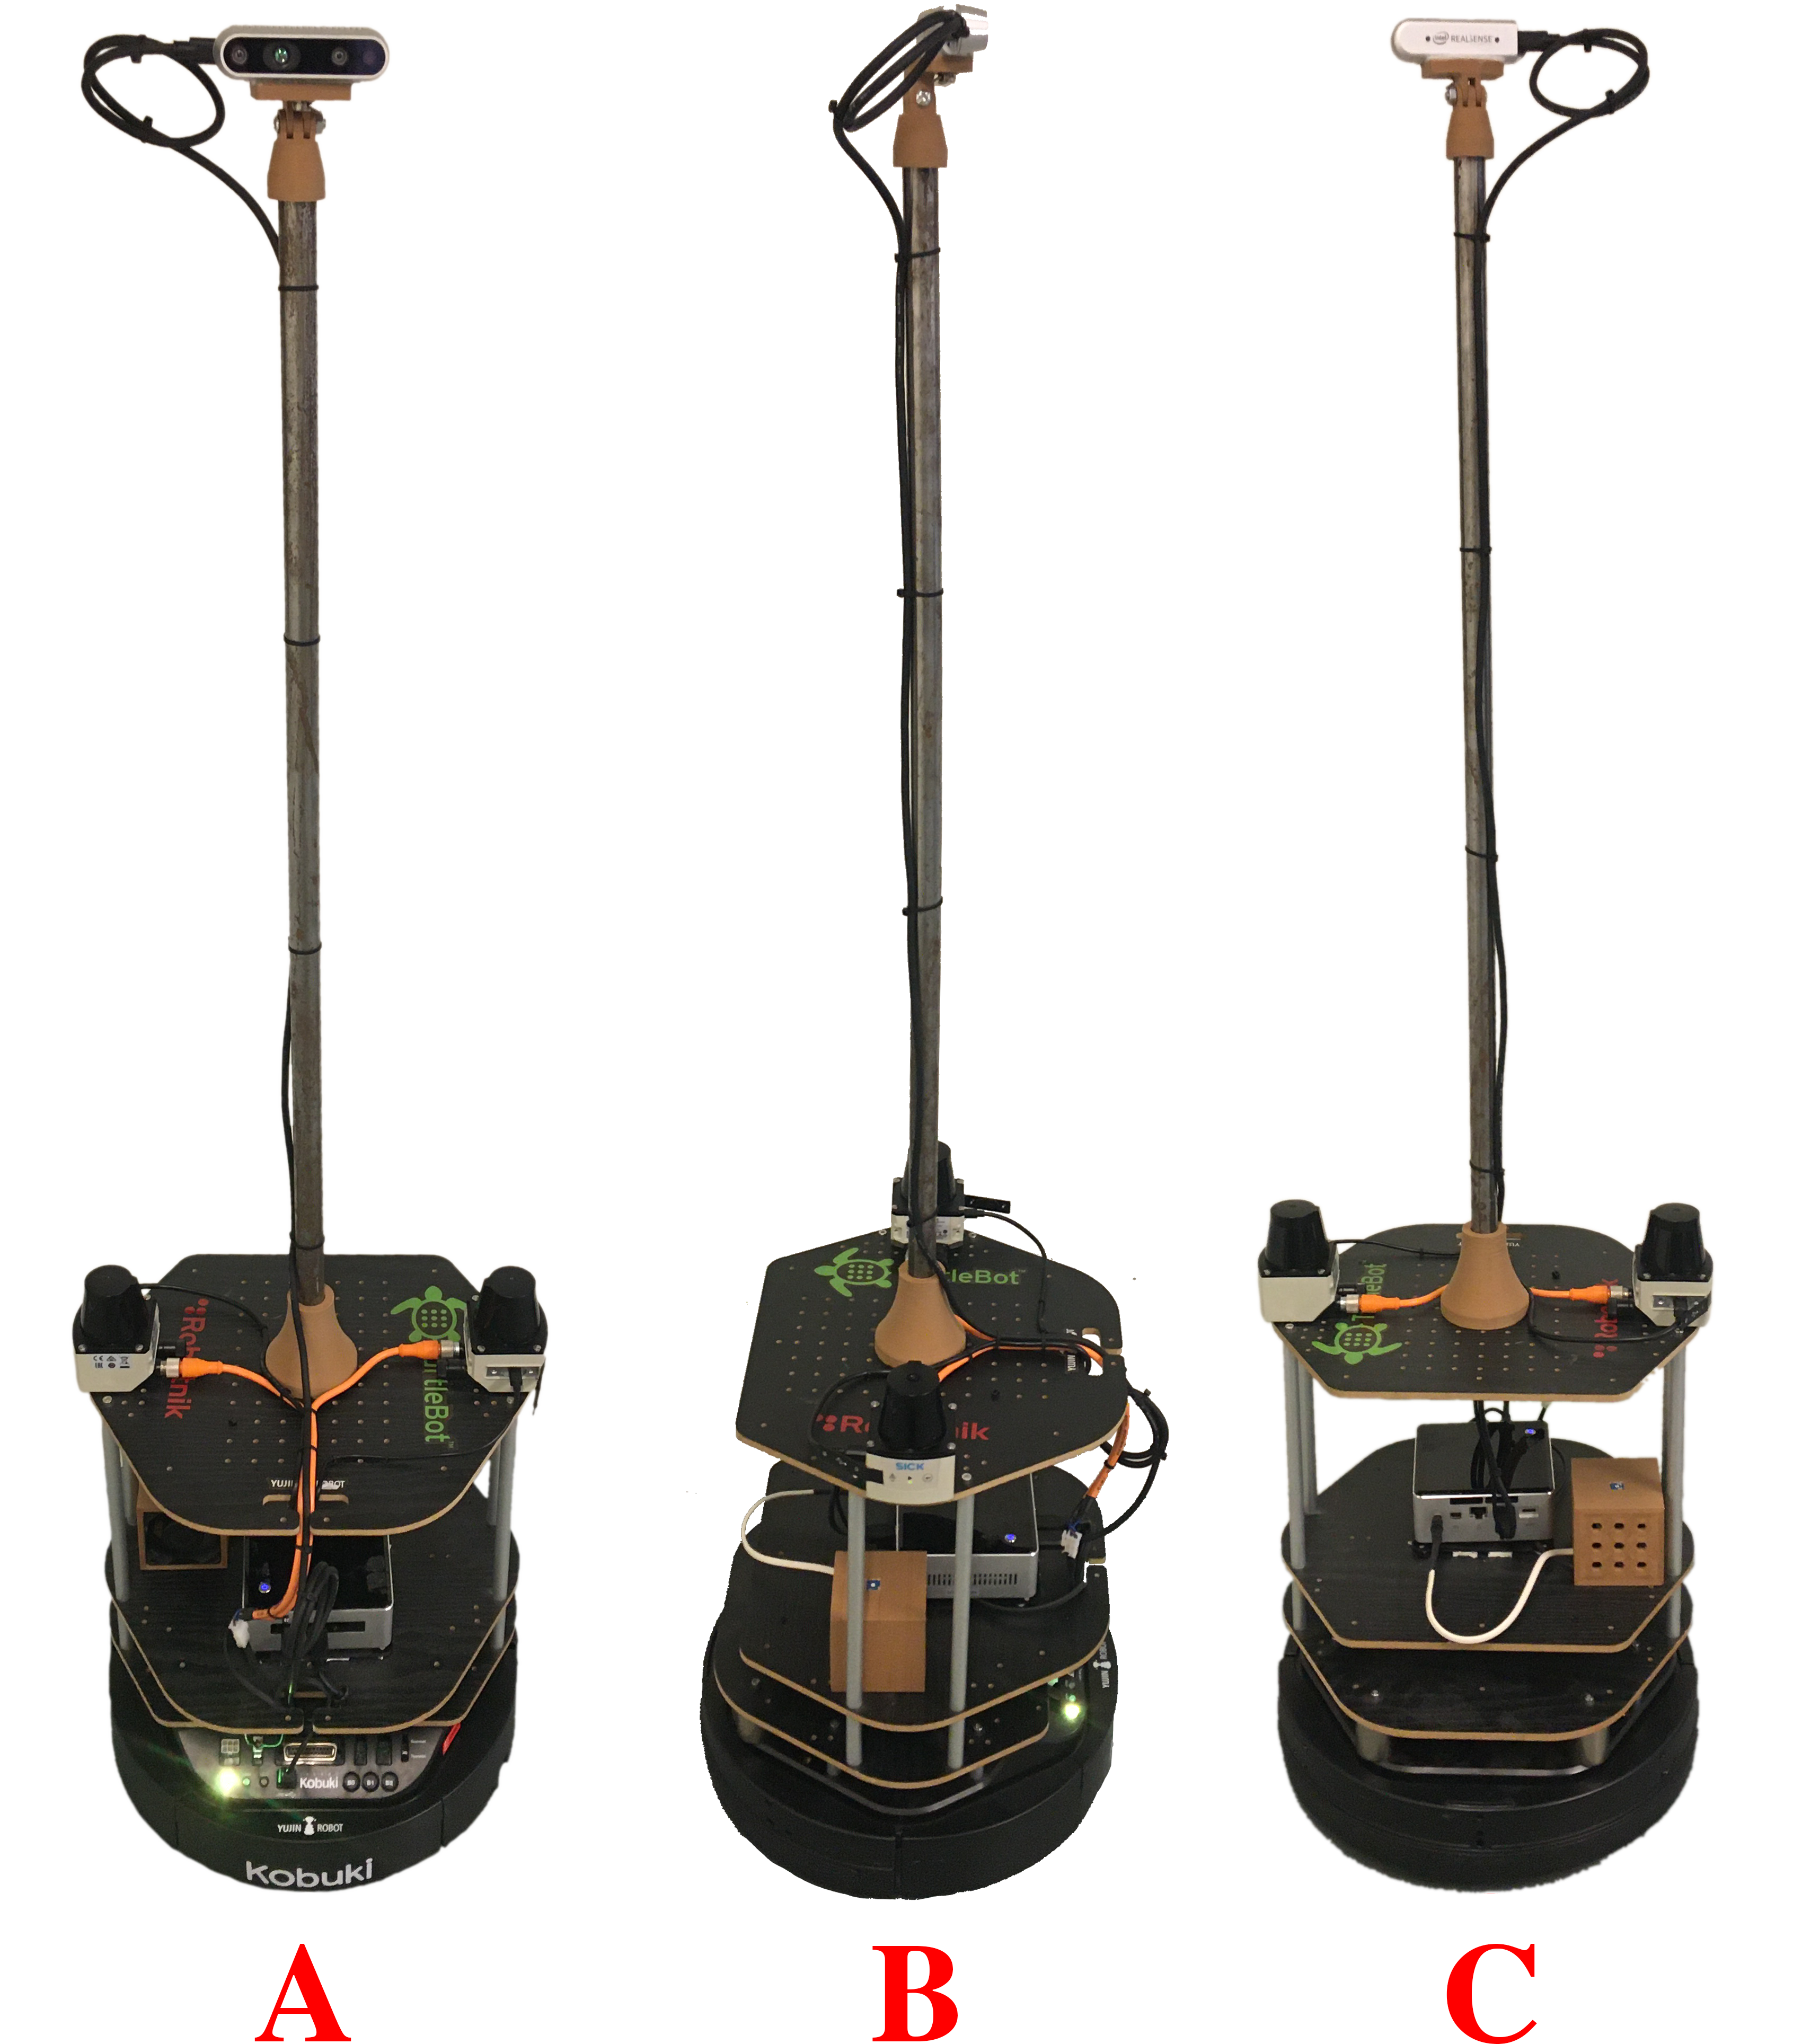
\includegraphics[width=.8\textwidth]{figures/TurtleBotFull.png}
    \caption{The physical prototype used for this project. A: The prototype seen from the back with the camera facing the user. B: The prototype seen from the side. C: The prototype seen from the front.}
    \label{fig:PhysicalSetup}
\end{figure}

The physical setup consists of the equipment previously described along with components to connect everything together. The main component for the connection of data streams from sensors is the NUC from intel. The NUC is a mini PC usable for many different purposes\cite{IntelNUC}. In this project the NUC is the main controller of the robot used to gather data from the sensors and do computations in order to determine the actions of the robot.\\

\begin{figure}[H]
    \centering
    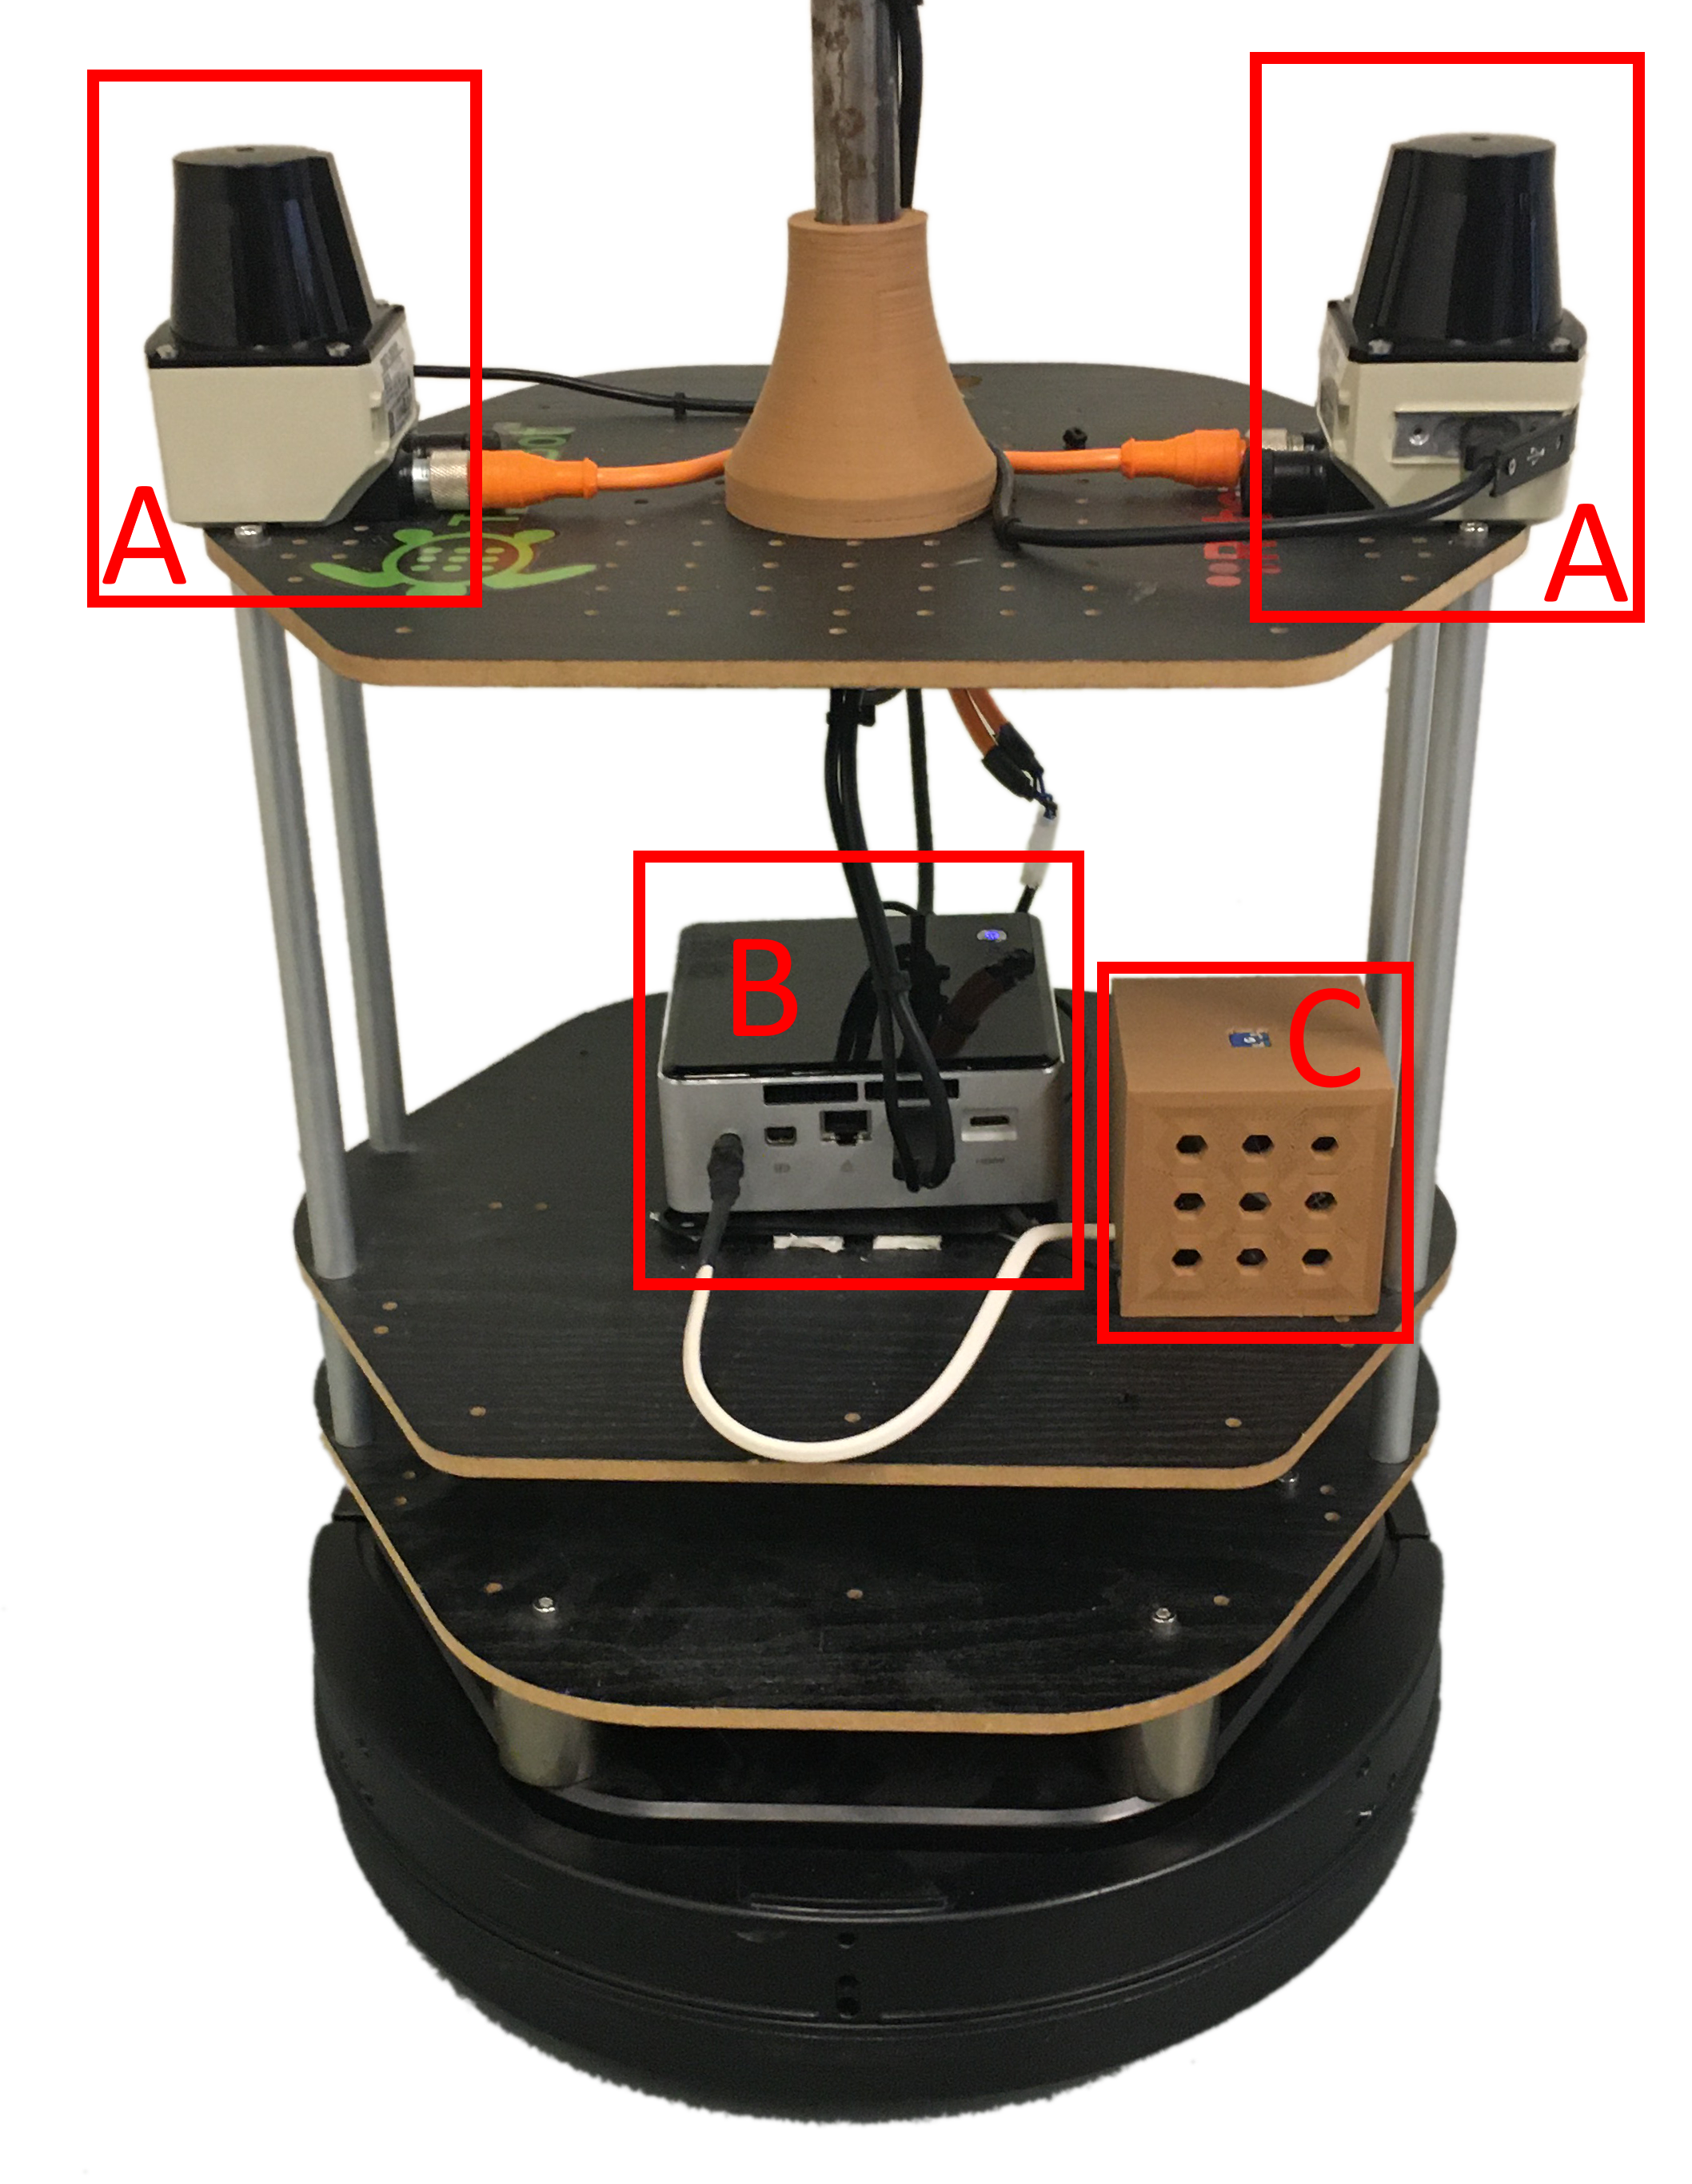
\includegraphics[width=.75\textwidth]{figures/Components.png}
    \caption{The components of the prototype. A: The SICK TIM571 LIDARS. B: The Intel NUC. C: Power convert for the Intel NUC.}
    \label{fig:Components}
\end{figure}

As can be seen in figure \ref{fig:Components}, the prototype carries all the needed components for this project. The LIDARS are placed on the top of the Turtlebot to be in the correct height for the leg detection, as described in section \ref{sec:height}. Additionally, the Intel Real Sense is mounted on a pole to put it in the correct height for facial detection as described in section \ref{sec:height}. In order to power the NUC from the Kobuki base, a power converter was made. This converter ensures that the NUC can run while the Kobuki base is turned on. Additionally, the battery level of the robot is monitored using one the LEDs of the Kobuki base. When the colour changes from green to yellow, the power is getting low. When the LED turns red the robot should be charged.\\
   
   \chapter{Software implementation}
%Add introduction to chapter
The software implementation chapter describes ROS (Robot Operating System) along with the implemented packages and algorithms. The first package that is looked at is the TF package that is used to transform the readings between the different sensors. The two major packages installed are leg\_detector and face\_detector, which are used to locate the people in proximity of the sensors. \\

The description of the robot and transformation between its coordinate frames are first used by specifying the placement of the different parts and their relationship. Then the depth image and laser scans are used for face detection and leg detection, respectively. They are used to keep track of the customer who uses a the robot in the hypermarket. The output of both detections are fused to give one Cartesian position of the person that is used for velocity control depending on the distance between the robot and the customer who is using it. The robot moves in the hypermarket by using the "move\_base" package. It uses the laser scan to localise itself in a known map and moves to a desired location in it while avoiding obstacles. If the customer is still following the robot, the robot keeps moving towards the desired location. This can be seen in figure \ref{fig:dia}.

\begin{figure}[H]
    \centering
    \includegraphics[width=1\textwidth]{figures/imp1.png}
    \caption{This flowchart describes how the implementation of the different data acquisitions, algorithms and sensors is done. The first process to be undergone is the URDF, so that the algorithm will know where the different sensors are located in relation to each other, then from the image and laser captures the two main algorithms will be run "face detection" and "leg detection". These two are running parallel and when outputs is received it will be fused so that a person might be perceived from this. When the person in the FOV is tracked a velocity control can begin, where the safe distance is described as in the social space, see fig \ref{fig:hall}, and MOVE\_BASE can commence. MOVE\_BASE uses the AMCL, which can be read about in the section about MOVE\_BASE. This MOVE\_BASE tracks itself in a map and should drive to the wares while avoiding obstacles. The last  implemented part is velocity control that ensures, the robot lowers its velocity or stops when the costumer following is not in the measured distance. This can be read in the section revolving the velocity-distance. If all of the above is successful then the guiding is undergoing or done.}
    \label{fig:dia}
\end{figure}

\section{ROS}\label{sec:ROS}
Robot Operating System (ROS) is an open-source software framework used for developing robotics software. It provides hardware drivers for a variety of sensors, and has a vast number of libraries, tools, and different algorithms that ease the task of programming robots, whether it is mobile robots or manipulators. It also provides visualisation and simulation tools. The core function of ROS is passing messages, which is done using publisher and subscriber communication paradigm.
Since ROS uses publisher and subscriber methods to exchange messages, a third component known as ROS master is used to filter and distribute the published messages to the corresponding subscriber.
Using ROS, processes communicate with each other through a peer-to-peer connection which is established by the ROS master. This network is known as ROS computational graph, where processes can be distributed across multiple machines or running on the same. ROS master keeps track of the running processes, also known as nodes, and handles name registration of them. ROS routes the messages published by the nodes to one another on a specific topic, where topics are named buses used for transferring data between nodes.\\
There are many reasons for using ROS, which include support for different programming languages such as C++, Python, Java, Lua and many others. Library integration is yet another advantage as many popular third-party libraries are supported such as OpenCV and Point Cloud Library (PCL). Scalability in the form of cloud computing is also possible using ROS in order to perform compute-intensive tasks. ROS also has tools for logging and playback of data in addition to tools for testing to find bugs in the code and to ensure its quality.\cite{ROScorecomponent}\\
A package this project has surrounded its algorithms around, is the "ros-people", and this package includes two different algorithms, such as "face-detection" and "leg-detection". However, before these algorithms can be dove into, a description of how the different sensors is placed is necessary.
   \section{TF package} \label{sec:tf_package}
The TF package is used to keep track of coordinate frames over time in a tree structure. It transforms points or vectors between two frames at any particular point in time. The Turtlebot has coordinate frames setup for the "base\_link" and its different sensors. The implemented design of the Turtlebot has a RealSense camera facing backward and two Sick LIDARs on the sides. The design can be seen in figure \ref{fig:robot_tf}.

\begin{figure}[H]
    \centering
    \includegraphics[width=\textwidth]{figures/robotTF.png}
    \caption{Figures are showing the base\_link, laser\_1, laser\_2 and camera\_link frames on the model of the Turtlebot from the front. Left figure is from the front. Right figure is from the side.}
    \label{fig:robot_tf}
\end{figure}

The camera and LIDAR frames have to be defined and established in TF to build a relationship between the different coordinate frames of the system. TF defines transformations between "parent" frame and "child" frame. Here, the parent frame is setup to be the "base\_link" of the Turtlebot, which is defined to be around the axis of rotation of the wheels. The child frame is the "laser" frame for the lidar and the "camera" frame for the camera. Since there are two LIDARs, the frames were called "laser\_1" and "laser\_2". The two LIDARs are parallel to each other and oriented away from each other on the Turtlebot. The frames are defined in $x$, $y$, $z$ and roll, pitch, yaw according to the right hand rule and the units are in SI units.


\begin{table}[H]
\centering
\begin{tabular}{@{}l|c|c|c|c|c|c|@{}}
\cline{2-5}
& \cellcolor[HTML]{DBDBDB}X & \cellcolor[HTML]{DBDBDB}Y & \cellcolor[HTML]{DBDBDB}Z & \cellcolor[HTML]{DBDBDB}Roll & \cellcolor[HTML]{DBDBDB}Pitch & \cellcolor[HTML]{DBDBDB}Yaw \\ \hline
\multicolumn{1}{|l|}{\cellcolor[HTML]{DBDBDB}Laser\_1} & 0.00 & 0.15 & 0.46 & 0.00 & 0.00 & $\pi$/2\\ \hline
\multicolumn{1}{|l|}{\cellcolor[HTML]{DBDBDB}Laser\_2} & 0.00 & -0.15 & 0.46 & 0.00 & 0.00 & $-\pi$/2\\ \hline
\multicolumn{1}{|l|}{\cellcolor[HTML]{DBDBDB}Camera\_link} & 0.00 & 0.00 & 1.30 & 0.00 & 0.00 & $\pi$\\ \hline
\end{tabular}
\caption{Table of coordinates relative to the base\_link, (x, y, z) represented in meters and (roll, pitch, yaw) in radians.}
\label{fig:coordiantetable}
\end{table}


The LIDAR laser frames are located 0.46 meters on the $z$-axis of the "base\_link" frame, oriented $\pm \pi/2$. Whereas the camera frame is 1.30 meters away on the z from the "base\_link" frame, oriented $\pm \pi$.

In the "turtlebot\_description" package, a new robot description were a added. This was done by first including macros that describe the different parts of the robot such as the Kobuki base, the hexagon plates that form the Turtlebot, the Intel Real Sense D435 camera as well as the SICK LIDARs. Afterwards, the different macros are defined by specifying, if needed, a list of parameters that were declared in the macro description of the part. Some of the parameters are the parent frame, x, y, or z offset in addition to roll, pitch and yaw for specifying the orientation between the frames of the parts in order to connect them in a TF tree structure.
   \section{ROS-people}
The ros-people package is a set of different ROS nodes that includes algorithms for detection of different parts of humans. These nodes can be connected and used for determination of a person's position in 3D space.\\

\subsection{Facial feature detection} \label{sec:Face}%detection 

To ensure detection of humans, multiple sensors will be used. One of these sensors is a camera that captures images in the average height of human faces to determine the presence of a person.\\

Calculating facial features can be computationally heavy due to the fact that many different features can be found on human faces. As the computer only perceives a face as a collection of pixels with different colour and/or light intensities it can be hard to detect a face, as shapes and sizes vary between different people.\\

To aid in the detection of faces, Paul Viola and Michael Jones created an optimisation algorithm, that utilises the Haar Classifier, that helps to quickly detect faces and other objects based on features known as Haar-like features\cite{Viola01robustreal-time}. These features use the change in contrast in rectangular groups of pixels to determine the relative dark and light areas of an object. A Haar-like feature contains two or three of these groups of relative contrast. The size of the examined pixel group can be increased or decreased in order to detect objects of different sizes. Different Haar-like features can be seen in figure \ref{fig:Haar-like}.

\begin{figure}[H]
    \centering
    \includegraphics[width=.6\textwidth]{figures/CommonHaarFeatures.png}
    \caption{Common Haar-like features that can be used to determine if an image contains a persons face.\cite{wilson2006facial}}
    \label{fig:Haar-like}
\end{figure}

Due to the vast amount of faces needed to train a facial detection program using a Haar Classifier, OpenCV trained libraries has been used for this project. These libraries have been trained on 10,000 images of faces of over 1,000 people along with 5,000 images of non facial images.\cite{wilson2006facial}\\

\subsection{Source Code}
The software for face detection can be found in appendix \ref{}.\\
The overview of the main code can be reviewed in the flowchart below, see figure \ref{fig:flowchartFaceMain}.
\begin{figure}[H]
    \centering
    \includegraphics[width=0.5\textwidth]{figures/main_face_flow.png}
    \caption{Flowchart of main loop of the face detection, that are implemented in this project. One important step in this flow chart is the loading of the cascade filters. The primary functions are the callbacks imagecallback() and depthimagecallback(), this is where the ROS message gets  converted to an image for use in openCV.}
    \label{fig:flowchartFaceMain}
\end{figure}

The face detector takes in a stream of images and depth images from the Intel Real Sense camera on the robot. This is done in two callback functions called in the function \texttt{faceDetector()}. The callback for the depth images is used to calculate the depth of the face if one is found. The callback of the image starts the procedure of detecting a face in the image by calling the function \texttt{detectAndDisplay()}.\\

The function \texttt{detectAndDisplay()} is the primary function for the face detection of this project, see figure \ref{fig:flowchartDetectface}.
This function takes the image from the camera and detects a face if one is present and combines the location of the face with the distance from the face to be transmitted to the tracking node.

To do this, \texttt{detectAndDisplay()} first converts the image from the camera to grey scale, due to the fact that the function detectMultiScale, which is utilised to detect faces and eyes only, works on a grey scaled image. To improve the detection speed of the function, the images are scaled down to have fewer calculations for every image. The ratio between width and height of the image is kept in order to ensure the shape of the faces.\\

With the scaled image, histogram equalisation is performed. This operation helps ensure similar looking faces in any lighting condition, to prevent faces from not being detected due to poor lighting. This is done by stretching out the histogram to make the captured image lighter and as seen figure \ref{fig:contrast}, then the features of the face can be seen more easily.
\begin{figure}[H]
    \centering
    \includegraphics[width=\textwidth]{figures/histogram.jpg}
    \caption{A visualisation of histogram equalisation. On the right is the original image. On the left is the image after histogram equalisation. The histograms below the images shows how the contrast changes between the images. The histogram is stretched out where the bins are taller to ensure a better contrast between different pixel values.\cite{histogram}}
    \label{fig:contrast}
\end{figure}

The histogram equalisation calculates a cumulative histogram of an image which is a slope of the pixel values of the image. With the cumulative histogram, the areas with a steep slope, i.e. where the pixel value is appearing often in the image, can be used to determine a new grey-level mapping for the image. This is done by mapping the high density bins of the histogram to a wider interval of pixel values while mapping the low density bins to a narrower interval. This helps ensure a better contrast of the image, resulting in more reliable use of the Haar Classifier.\cite{imagebook}\\

Then, to perform the detection and classification of Haar-like features, OpenCV's \texttt{CascadeClassifier.detectMultiScale()} is used. With the features calculated, any face in the image should be detected.
The detection is done by applying different Haar-like features to the image to determine if any fit an area. If there is a positive match between the feature and the area, the cascade will continue trying different features to narrow down the area of a face. When an area of a face is narrowed down many different Haar-like features are compared to determine the match of a face. This can be seen in figure \ref{fig:Haar-featureFace}

\begin{figure}[H]
    \centering
    \includegraphics[width=0.8\textwidth]{figures/LenaHaarFeatures.jpg}
    \caption{The figure shows different Haar-like features applied to a face. These are applied at different stages to determine the presence of a face. If multiple features are not present the classifier will determine the likelihood of a face to be low and therefore, not classify it as such. In the figure both line features and edge features are shown.\cite{LenaHaarFeatures}}
    \label{fig:Haar-featureFace}
\end{figure}

The function detectmultiscale also gives a score the detected face in the image, there is also an adjustable value named neighbouring faces. The neighbouring faces is not how many faces is in the given image, when a face with Haar-cascade filter, as it is possible that a larger square or a shifted square has obtained the same image. The square with the larges scores is returned, meanwhile the other squares are considerate neighbouring faces.
\begin{figure}[H]
    \centering
    \includegraphics[width=0.6\textwidth]{figures/callback_face_flow.png}
    \caption{Flowchart of face and eye detection function implemented in this project. The two functions are described in there separate flowchart. The function detectAndDisplay and are described in flowchart later in this section, see figure \ref{fig:flowchartDetectface}}
    \label{fig:flowchartCallbacks}
\end{figure}


%Insert image of detected face


 With the detection of the face, the position of the face in the image is calculated. This can be used to determine the centre of the face for further use for detecting the position of the person as well as detect facial features. To further ensure that the detected face is indeed a face, eye detection is performed on the original image within the boundaries of the face previously calculated. The detection is done on the non-scaled image due to the size of eyes being too small in a down scaled image. Both the face- and the eye recognition can be seen on figure \ref{fig:detectedfaces}. 

\begin{figure}[H]
    \centering
    \begin{minipage}[b]{0.5\linewidth}
   Here two faces are detected and a circle is drawn from the centre of the face in pink, and the eye is drawn in the same fashion. Only one eye is detected, this is due to the high illumination of on the right side of the faces.\\
   About how the different callback functions work can be reviewed in figure \ref{fig:flowchartCallbacks}, and figure \ref{fig:flowchartDetectface}.
    \end{minipage}
    \hspace{0.2cm}
    \begin{minipage}[b]{0.47\linewidth}
    \includegraphics[width=\textwidth]{figures/detecedFace.png}
    \caption{The face- and eye detection, detecting two faces.}
    \label{fig:detectedfaces}
    \end{minipage}
\end{figure}



\begin{figure}[H]
    \centering
    \includegraphics[width=0.8\textwidth]{figures/color_face_flow.png}
    \caption{Flowchart overview of the workings of the callback functions implemented in this project when a image message is received.}
    \label{fig:flowchartDetectface}
\end{figure}

With the face detected the position of the face in the image is used to extract the distance and angle to the person relative to the robot. The distance and angle are converted into an x and a y coordinate of the person. To see a visual representation of this, see figure \ref{fig:lidscan}. The angle is found by centre point of face in the detectmultiscale and maps the point between -1.0 and 1.0 and multiplied with the half width of cameras FOV in degrees
    

\begin{figure}[H]
    \centering
    \includegraphics[width=0.7\textwidth]{figures/cameraview1.png}
    \caption{A visual representation of how the facedetector calculates the x-y coordinate of the persons tracked, where the dotted line is the length from the camera.}
    \label{fig:lidscan}
\end{figure}


Along with a ROS timestamp in the headers the xy coordinates is transmitted in a ROS-message to be used by the Kalman Filter for tracking of the person to be guided, described in section \ref{sec:KalmanFilter}.

The Kalman filter needs the covarince of the sensors. The covariance in this node is implemented as a variation over time, E.g the Cartesian xy coordinates is taken from each frame, that are captured of a person.
The mean or the sample mean which are implemented in this node, is because it is not possible to get a population mean, due to dropped data. 

The sample mean is calculated as so, where $\bar{x}$ is the sample mean of x.
\begin{equation}
    \bar{x} = \frac{1}{n-1} \times \sum_{n=1}^{25}x
    \label{eq:sampleXmean}
\end{equation}
\begin{equation}
    \bar{y} = \frac{1}{n-1} \times \sum_{n=1}^{25}y
    \label{eq:sampleYmean}
\end{equation}

From there the estimated variance of the x and y coordinates are calculated like so: where $\hat{\sigma_{x}}, \hat{\sigma_{y}}$ is the estimated sample variance
\begin{equation}
    \hat{\sigma^{2}_{x}} = (x - \bar{x}) \times (x - \bar{x})
    \label{eq:sigmaX}
\end{equation}
\begin{equation}
    \hat{\sigma^{2}_{y}} = (y - \bar{y}) \times (y - \bar{y})
    \label{eq:sigmaY}
\end{equation}

The estimated variance between y and x, also known as the covariance,
is calculated in the same manner with a slight difference.
\begin{equation}
    \hat{\sigma^{2}_{xy}} = (x - \bar{x}) \times (y - \bar{y})
    \label{eq:sigmaXY}
\end{equation}

Each calculation of the variance, $\sigma^{2}_{x}$ , $\sigma^{2}_{y}$and $\sigma^{2}_{xy}$, equations  \ref{eq:sigmaX},\ref{eq:sigmaY} and \ref{eq:sigmaXY} is based on the new x and y coordinate and sample mean.
The sample mean are calculated over a period of 25 frames, of the tracked person, an example can be seen in figure \ref{fig:varMean}. If only five frames has passed since the person is being tracked, the sample mean will only be calculated over the period of the five frames instead of 25 as seen in \ref{eq:sampleXmean}, \ref{eq:sampleYmean}. So there will be a period where the variance may fluctuate more than after the 25 frames are captured. Figure \ref{fig:varMean} depicts the implementation of the calculation of the variance.

\begin{figure}[H]
    \centering
    \includegraphics[width=\textwidth]{figures/mark2.png}
    \caption{This illustration of how the implementation of the variance of the xy coordinate. The face moves over time, the dots are the measured point of the persons, the red dot shall be seen as the average of the measurements, this is being translated to a variance in this example the variance of x. The $\sigma$ is the std. deviations, this can used to interpolate how far from the norm the measurement of x are.}
    \label{fig:varMean}
\end{figure}

%The face detector uses openCV to detect faces through stereo camera data. Haar-like features is used to get an initial set of detections, these features is based on change in contrast. A Haar group is formed if the detections line three or more adjacent pixels up with the necessary contrast values \cite{wilson2006facial}.
%The face detector then removes the false-positives by using the depth to predict the size of the head. Objects larger than the prediction will then be pruned.\\
%The face detector can be used as a continuous stream of data or as an action, where it will process the images until it has found at least one face. The action results is a list of faces found, the list is named face\_positions under people\_msgs/PositionMeasurement. It subscribes to the topic people\_tracker\_measurements, which contains the 3D position of the center of the face \cite{facedetect}.
   \subsection{Leg detection} \label{sec:LegDetect}
Leg detection is used to calculate the geometry of legs and apply these calculation in a way so that a person's centre can be found. An overview can be viewed in figure \ref{fig:legflow}.
\begin{figure}[H]
    \centering
    \includegraphics[width=.6\textwidth]{figures/leg2.png}
    \caption{Overview of the leg detection algorithm}
    \label{fig:legflow}
\end{figure}

%features:
The leg detector converts a number of points, or clusters, in the image into readable matrices for the OpenCV program. These matrices are then used to identify features, which is used to determine the reliability for the leg detection. Some of the features are:

\begin{itemize}
    \item Circularity
    \item Width
    \item Radius
    \item Mean angular distances
\end{itemize}

The reliability decides whether the tracked object is a person or not. These features establishes the foundation of a single leg and later on in the algorithm these legs are paired to connect them as persons. However, two table-legs can also be tracked but the width and radius often makes them displayed as false-positives, which will appear as blue dots when the tracker is visualised in RViz. And the people detected as persons will appear as a green dot with 2 red dots on each side, which is the legs as seen in figure \ref{fig:rviz}. RViz is a tool used to run visualisation of a robot.\\

\begin{figure}[H]
    \centering
    \includegraphics[width=0.8\textwidth, height=10cm]{figures/rviz.png}
    \caption{Visualisation of the leg detection in RViz. The dark-blue dots are false-positives and the green dots are perceived as humans, while the red dots are perceived as legs}
    \label{fig:rviz}
\end{figure}

In this algorithm there is 3 files worth mentioning, the first is the training.cpp. This file includes the data read from the camera and it tries to continuously classify the different aforementioned features so that the code can keep running. However the training.cpp is also continuously trying to reduce the computational power, much like the HAAR cascade, see section \ref{sec:Face}, by only looking for the aforementioned clusters. If only false-positives or no clusters is in the LIDARs field of view the code will only run this section of the code and the computation is reduced.\\
The second file is the feature\_extraction.cpp, which has briefly been touched upon by stating which features it scans for and how the points gathered from the LIDAR is converted to a readable matrix to use with OpenCV.\\
The third file is the leg\_detector.cpp and this file is where the actual leg detection happens. A combination of geometry messages and tracking of the leg is implemented in this file. However the first thing to establish is that each leg is provided with a time-stamp when it has been tracked and this time-stamp will serve as constant in a function that measures the walking patterns or speed of the tracked humans.\\
The leg\_detector algorithm tracks people by following a single rule for the legs, the distance between the legs. An estimate of the average distance between the legs of a person has been found and the writers of the algorithm has established that this number is between 20 to 50cm. When each feature has been reasonably close to resemblance of a leg the tracker stamps it and then it continuously looks for other legs in the perimeter of 20 to 50cm. If another leg is found it will ID these legs as person and the readings of the leg detector will be published so that position, time-stamps, IDs, and reliability, etc. can be surveilled, as seen in figure \ref{fig:reliability}.

\begin{figure}[H]
    \centering
    \includegraphics[width=\textwidth]{figures/leg_detector_msg.png}
    \caption{The message structure of the leg detection, published on the topic /legdetector}
    \label{fig:reliability}
\end{figure}

However one measurement is not mentioned and that is the covariance. The covariance is an array that utilises geometry messages to establish the relations between the values of the position messages and that of the reliability score. In the position messages the authors of the code include several measured values to get a reasonable covariance value. %line 880 in the code
With these detection measurements available human legs can be tracked and connected with the aforementioned face-id.\\
   \section{Kalman Filter} \label{sec:KalmanFilter}
This section describes the theory behind and implementation of a Kalman filter used for sensor fusion and tracking of a person in this project.\\

The sensors described in chapter \ref{ch:equipment} measure data with some noise, giving readings that are not completely reliable. Additionally, as more sensors are used to track the same person, these must be fused, using an algorithm, in order to ensure the best estimate of the position of people. Both the fusion of sensors and reduction of noise in measurements can be achieved by implementing a Kalman filter for tracking people.\\

The Kalman filter supplies a recurring method for estimating the state of a dynamic system when the system contains noise. The Kalman filter maintains estimates of the state vector ($\hat{x}$) and the error covariance matrix ($P$) of the system. This assumes that the system has a Gaussian probability density function (PDF) as an output with the mean $\hat{x}$ and covariance $P$. In the context of tracking people this means that the estimated position, calculated using the Kalman filter, is a distribution of likely positions rather than a particular position.\\

%Insert some picture if it makes sense

As mentioned previously, the Kalman filter is a recurring function running in two steps, prediction and update. The first step, prediction, takes the known parameters of the system to estimate the current state of the system $\hat{x}(k+1|k)$ along with the covariance propagation $P(k+1|k)$. With the predicted state of the system calculated, the sensor measurements can be compared to the prediction to compute the updated state of the system. This is done in the update step where the Kalman gain ($K$) is computed based on the estimated covariance and the sensor noise. The Kalman gain is then used to compute the updated state of the system by combining the predicted state with the sensor measurements to determine the new Gaussian PDF for the time step ($k+1$). The Kalman gain is used to determine the weighted average of the prediction and the measurements, dependant on the uncertainty of each value.\cite{choset2005principles}

\subsubsection{Prediction step}
As described above, the prediction step predicts the state and covariance of the system. This is done in the following two functions:

\begin{equation}
\hat{x}(k+1|k) = F(k)\hat{x}(k|k)+u(k)
\end{equation}
which is the prediction of the mean of the position and,
\begin{equation}
P(k+1|k) = F(k)P(k|k)F(k)^T+Q(k)
\end{equation}
which is the prediction of the covariance of the position.

Where:
\begin{itemize}
    \item $\hat{x}$: Estimation vector
    \item $k$: Kalman gain
    \item $F$: The state transition matrix
    \item $u$: Control vector adding any known changes to the system 
    \item $P$: Prediction matrix
    \item $Q$: Overall process noise in a covariance matrix.
\end{itemize}
\vspace*{5mm}

%where \textit{F} is the state transition matrix, depicting the base change of \textit{x} and \textit{P}, and \textit{u} is the control vector adding any known changes to the system (such as a change in velocity of the observer).

%where \textit{Q} is an overall process noise in a covariance matrix.

\subsubsection{Update step}
The update step combines the prediction with the sensor measurements as described previously. This is calculated in the following two functions:
\begin{equation}
\hat{x}(k+1|k+1) = \hat{x}(k+1|k) + Ky
\label{eq:kalmanupdate1}
\end{equation}
which is the updated mean of the position and,
\begin{equation}
P(k+1|k+1) = (I - (K * H(k+1)) P(k+1|k)
\label{eq:kalmanupdate2}
\end{equation}
which is the update of the covariance of the position.

Where:
\begin{itemize}
    \item $y$: Measurement residual
    \item $I$: Identity matrix 
    \item $H$: Vector mapping matrix
\end{itemize}
\vspace*{5mm}

%where \textit{K} is the Kalman gain and \textit{y} is the measurement residual, the difference between measured and expected values.

In both equation \ref{eq:kalmanupdate1} and \ref{eq:kalmanupdate2}, the $K$ is calculated by $K=PH(k+1)^TS^{-1}$, where $S$ is a residual covariance matrix that is increased by measurement noise. Additionally, the $y$ is calculated $y = Z(k+1)^T - H(k+1)x$, where $Z$ is measurements from the sensors.\\

With the general description of the Kalman filter concluded, the implementation of the filter for this project can be explained.

\subsection{Implementation of the Kalman Filter}

The Kalman filter is used for fusing the data from the leg detection and face detection in this project and publishing the data to the implemented velocity controller.
The Kalman filter is implemented through the use of a python library called pykalman\cite{pykalman}. This is the reason for the ROS node Kalman filter being written in python rather than in C++ as the other nodes.
The pykalman needs six initiations matrices, transition ($F$), observation ($H$), transition covariance ($Q$), initial observation covariance ($R0$), initial estimation ($X0$) and initial prediction ($P0$), this is called every time a new Kalman filter object is created. This Kalman filter is implemented in such a way that it works best on updating it with a approximately same time step, meaning updating the filter at frequency, with or without new measurements. This requires The ROS node to run at a frequency that is able to handle data, published at different frequencies, this is done be updating at higher frequency than is published on any of the topics. To ensure that if data arrives at the same time a boolean is used to only allow one update per time step. If the Kalman filter updates without any new measurements from the two topics, it will update on the previous estimate of the person and prediction made.\\

\begin{figure}[H]
    \centering
    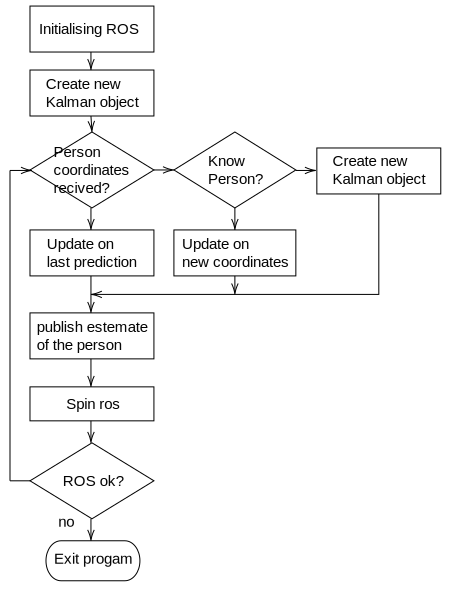
\includegraphics[width=0.65\textwidth]{figures/flow_pykalman.png}
    \caption{Flow chart of implementation of node running the Kalman filter}
    \label{fig:flow_pykalman}
\end{figure}

When a person is first detected on the leg detection topic, it stores the persons data. A helper class is created to hold the values of the persons evaluated, i.e the x,y coordinates and a name. The name of the person that is received from the leg detector node, to compare if it is a new person or if it is the same as previous detected. If the person is the same it will update the Kalman filter with the $k-1$ estimate of position, the $k-1$ prediction, the observation and the observation covariance. The new updated estimate of the x and y position from the Kalman filter is published to the speed controller. If it is a new person that has been discovered a new initialisation of the Kalman filter is created, as previous mentioned with initial matrices.\\
If a message is received on the face detector topic, the Kalman filter will only update the Kalman filter with the received data due to the way of implementation of the face detector. The face detector does not check if the image that it analyses is the same person. Every time this node filters and publishes it is done through the same method in the class that is named Kalman in this project. This method is named filter and pub, it requires two arguments to be passed to the observation and the covariance observation. These arguments are used to update the Kalman filter, if there is no new input from the sensors, the keyword none is passed in as the observation and observation covariance, to make the Kalman filter only update in the previous estimate and prediction. This method keeps track of the time and ensures that the update frequency and the new estimate is published correctly, by the use of rospy.sleep function, that is set to the specified rate, and rospy.spin.
   \section{Move\_base} \label{sec:move_turtlebot}
To move the Turtlebot around in a hypermarket, the "move\_base" package is used. This package allows moving a mobile base to a desired goal in the world. By default recovery behaviours are performed when the robot is stuck which can be necessary as hypermarkets are semi-structured environment where many dynamic obstacles can be in the way. These behaviours are seen in figure \ref{fig:move_base}.\\

\begin{figure}[H]
    \centering
    \includegraphics[width=0.9\textwidth]{figures/recovery_behaviors.png}
    \caption{Move\_base recovery behaviour.}
    \label{fig:move_base}
\end{figure}

The "move\_base" package allows the user to adjust many parameters the robot uses in its attempt to achieve a goal within a user-specified tolerance. These parameters can be changed on run-time using the parameter server. The "move\_base" package contains other key components for navigation like the "base\_local\_planner" package. This package uses algorithms connecting path planning to the robot by the use of a controller that generates velocity commands providing a map. The idea of these algorithms is as follow:

\begin{enumerate}
    \item Sample the linear velocities along x, y and the angular velocities along theta.
    \item Forward simulate each sampled velocity from the current state of the robot to predict the effect of applying this velocity for a period of time.
    \item The trajectories resulting of the forward simulation are scored according to different metrics that incorporates things such as distance to obstacle, goal and global path as well as speed. Trajectories that collide with obstacles are discarded.
    \item The trajectory with the highest score are chosen and the corresponding velocity is sent to the mobile base.
    \item Repeat.
\end{enumerate}

\begin{figure}[H]
    \centering
    \begin{minipage}[b]{0.57\linewidth}
    Figure \ref{fig:trajecories_mobileBase} shows trajectories simulated by a mobile base in order to determine which one has the highest score.\\
    Optionally, the "move\_base" package uses AMCL (Adaptive Monte Carlo Localisation) in order for the robot to localise itself in a map. This package uses filters to determine the pose of the robot in a known map.
    In order to keep a specific distance from the person being guided through the hypermarket, the velocity of the robot along with other metrics need to be changed dynamically.
    \end{minipage}
    \hspace{0.2cm}
    \begin{minipage}[b]{0.4\linewidth}
    \centering
    \includegraphics[width=\textwidth]{figures/local_plan.png}
    \caption{Mobile base with simulated trajectories to determine which path has the highest score.}
    \label{fig:trajecories_mobileBase}
    \end{minipage}
\end{figure}

The implemented node sends a goal to the action server by using an action client. This way of requesting the robot to move allows getting periodic feedback about the progress of the moving task, where three messages are used to communicate between the server and the client. These messages are Goal, Feedback and Result. In this case, the goal is a geometry message of type PoseStamped, that is defined by a position, orientation as well as a time stamp. The Feedback contains a PoseStamped message indicating the current pose of the robot in addition to GoalStatus message which is defined by unsigned integer values indicating the progress of the robot in completing the requested goal, being pending, active, aborted, succeeded or lost, among other status. The Result is GoalStatus message as well that is sent from the server to the client when the goal is completed, however, it is only sent once.\\

A graphical user interface were implemented by using a library called GTKMM to allow the customer to send a goal to the action server. The interface consists of 100 buttons with different labels indicating the different wares of the store, each buttons corresponds to a position on the map of the store. The buttons are arranged in a grid of 10 by 10 which is added to a scrolled window. The interface can be seen in figure \ref{fig:move_gui}.

\begin{figure}[H]
    \centering
    \includegraphics[width=0.9\textwidth]{figures/gtkmm_gui2.png}
    \caption{A graphical user interface showing different buttons that correspond to different wares of a store.}
    \label{fig:move_gui}
\end{figure}
   \section{Velocity Controller}\label{sec:velocity_controller}
The velocity controller node uses a linear function that is inversely proportional, which means that the function's product will be unchanged, to the distance from the customer who is using it. This means that the further the customer is away from the robot, the slower the robot will move to let the customer catch up to it. Equation \ref{eq:velocityFunction} shows the line function of the controller.

\begin{equation}
    Velocity = -(0.38 * distance\_from\_person) + 1.16
    \label{eq:velocityFunction}
\end{equation}

The line function were found by using two points that define the behaviour of the velocity controller. Point A(1.2, 0.7) where 1.2 defines the minimum distance to keep from the person and 0.7 defines the maximum velocity of the robot. Point B(3.0, 0) is the maximum distance between the robot and the person, and 0 is the velocity of the robot at that distance. Figure \ref{fig:velocity_controller_graph} shows a graph of the line equation.

\begin{figure}[H]
    \centering
    \includegraphics[width=0.9\textwidth]{figures/velocity_distance_graph.png}
    \caption{Graph showing the relation between the velocity of the robot and the distance from the person.}
    \label{fig:velocity_controller_graph}
\end{figure}

The node works by first subscribing to "sensorPosition" topic which is the output of the Kalman filter. The output is a point in the map indicating where the tracked person is in xy-plane. This point is then used to calculate the distance to the person from the "base\_link" frame of the robot. The velocity is then calculated and sent to the parameter server using the "dynamic\_reconfigure" package. If the distance to the customer is greater than 3 meters, the robot sends a request to the "move\_base" action server to cancel the current goal and the robot stops in place.
  
   \chapter{Testing}\label{Testing}
A prototype or proof-of-concept can be difficult to use as a selling point, without proof that the product works. Scheduling tests for different parameters of the product can help improve the credibility by showing that different parts of the product works and documenting the strengths and weaknesses of it.


\section{LIDAR Accuracy test}
Testing the equipment of the system is important, as it may impact how the system functions as a whole. This test will test the error margin of the LIDARs, by reading the distance from the LIDAR to the distance of an object.\\

\textbf{Equipment}: The equipment used is a SICK TiM571 LIDAR, measuring tape, a cardboard and software to read distances measured from the LIDAR.\\
    
\textbf{Setup}: The LIDAR is placed in a corner with 5 meters of free space in a 10 degree angle. This is to help leave out the things the LIDAR should not be measuring distance to. Lines were drawn on the floor that had a distance relative to the middle of the LIDAR, as if the LIDAR was placed on the floor (currently it is mounted on the robot). Two people, person A and person B have each their job. Person A holds a piece of cardboard that is placed orthogonal to the LIDAR, see on figure \ref{fig:AccuracySetup1}, on the marked spots that had a distance of 0.5m, 1m, 1.5m, 2m, 2.5m, 3m, 3.5m, 4m, 4.5m relative to the LIDAR, see figure \ref{fig:AccuracySetup2}. Person B has to read the distance, information read on the computer that comes from the LIDAR software.

\begin{figure}[H]
    \centering
    \begin{minipage}[b]{0.5\linewidth}
        \includegraphics[width=\textwidth]{figures/AccuracySetup1.jpg}
        \caption{Person A holding the cardboard piece at a distance of 0.5m from the LIDAR. The 0.5m mark made with the white chalk is barely visible at the bottom of the board.}
        \label{fig:AccuracySetup1}
    \end{minipage}
    \hspace{0.2cm}
    \begin{minipage}[b]{0.45\linewidth}
        \includegraphics[width=\textwidth]{figures/AccuracySetupPs.png}
        \caption{The position of the robot and LIDAR, with white spotted lines placed on top  of the chalk lines that have been drawn on the floor, marking the distance to the LIDAR with an increment of 0.5m for each line.}
        \label{fig:AccuracySetup2}
    \end{minipage}
\end{figure}

% \begin{figure}[H]
%     \centering
%     \includegraphics[width=0.75\textwidth]{figures/AccuracySetup2.png}
%     \caption{The position of the robot and LIDAR, with white chalk lines marking the distance to the LIDAR, if it was placed on the floor. This was done as it is difficult to mark distances at the same height as the LIDAR.}
%     \label{fig:AccuracySetup2}
% \end{figure}


\textbf{Execution}: Person A held the piece of cardboard at the marked distances, starting from 0.5m all the way to 4.5m at 0.5m increments. When person A thought the cardboard was placed at the exact marked spot and held vertically, he let person B know, who then denoted the distance read from the LIDAR. Person B only denoted the distance when person A told him to, to achieve the best distance. Person A was fiddling the cardboard when placing on the chalk line, and Person A knows when the board is in the right place.\\
Person B would look at the stream of distance data and take the average of the next three incoming data lines, see figure \ref{fig:AccuracySetup3}. The smallest distance measured by the LIDAR was published, hence why it was important to use a small angle in an empty room. person B would also look at the program RViz, which was also used on the sideline to make sure nothing else was causing readings, other than the cardboard.\\

% \begin{figure}[H]
%     \centering
%     \includegraphics[width=0.45\textwidth]{figures/AccuracySetup1.jpg}
%     \caption{Person A holding the cardboard piece at the 0.5m point. The white chalk is barely visible at the bottom of the board.}
%     \label{fig:AccuracySetup1}
% \end{figure}

\textbf{Test Parameters}: The incoming data stream from the LIDAR for each distance from the cardboard to the LIDAR. Only 2 decimals were used, as from the third decimal, were changing too quickly to read. 

\begin{figure}[H]
    \centering
    \includegraphics[width=1\textwidth]{figures/AccuracySetup3.png}
    \caption{The software that streamed the shortest distance read by the LIDAR. Person B used this to determine the distance, when person A said he was in position with the cardboard.}
    \label{fig:AccuracySetup3}
\end{figure}

\textbf{Results and analysis}:
\begin{center}
 \begin{tabular}{||c c c||} 
 \hline
 Marked distance & Measured Distance & Error percentage \\ [0.5ex] 
 \hline\hline
 0.5m & 0.5m & 0\%\\ 
 \hline
 1m & 1m & 0\%\\
 \hline
 1.5m & 1.49m & 1\%\\
 \hline
 2m & 2m & 0\%\\
 \hline
 2.5m & 2.51m & 0.4\%\\
 \hline
 3m & 3.02m & 0.6\%\\
 \hline
 3.5m & 3.5m & 0\%\\
 \hline
 4m & 4.01m & 0.2\%\\
 \hline
 4.5m & 4.5 & 0\%\\ [1ex] 
 \hline
 \label{table12}
\end{tabular}
\end{center}
Table \ref{table12} shows the results of the accuracy test. The error percentage averages 0.22\% throughout 9 readings at distances from 0.5m to 4.5m. This is so small it is not only irrelevant but points towards imperfections with the test setup. As the distance markings were done by hand, with measuring equipment, there is a chance of inaccuracies. Same goes for holding the cardboard at the exact mark and the right angle. The error margin of the error is 20mm according to SICK themselves.\\ %REF here

\textbf{Sources of error}:
\begin{itemize}
    \item The SICK TiM571 LIDAR has an error margin of 20mm.\cite{timerrormargin}
    \item The cardboard was held by hand, and might not be held in the correct angle at all times. Small movements would be caught on the readings and may be the reason for the average result be a little incorrect.
    \item The chalk lines on the floor have been drawn manually and there may have been a slight movement when drawing the lines, making a small mistake in where the cardboard would be placed when doing the readings.
\end{itemize}

\section{Leg detection test}
%This test serves to gain knowledge about the reliability of the leg detection system used for this robot. 
This test serves to gain knowledge about the reliability of how the LIDARS work with the software written for the leg detection. It is important to know the capabilities and limits of a system, especially when moving a robot in dynamic environments with humans. It was also used to decide whether one LIDAR detecting a person is enough or if both LIDARs need to confirm it simultaneously within a 1cm devation between the LIDARs.\\


\textbf{Equipment}: The equipment used when conducting this test consists of two Sick TIM571 LIDARs, ROS People's package, a room with 5 meters * 5 meters grid marked on the floor and two test persons.\\

\textbf{Setup}: The robot is located in the corner of the 5m*5m grid marked on the floor, angled towards the diagonally opposite corner, see figure \ref{fig:LidarCoverage}. 

\begin{figure}[H]
    \centering
    \includegraphics[width=0.85\textwidth]{figures/LidarCoverage.png}
    \caption{A visual representation of the LIDARs covered area when limited to 5m.}
    \label{fig:LidarCoverage}
\end{figure}

This is because the space in a 90 degrees angle behind the robot is what we are most interested in using to detect people. Test persons will take turns standing twice, with two different poses, in specific quadrants and the person detection will be noted (false or positive). The layout is shown in figure \ref{fig:LidarCoverage} and \ref{fig:LegDetectorSetup}. 

\begin{figure}[H]
    \centering
    \includegraphics[width=0.85\textwidth]{figures/LegDetectorSetup.png}
    \caption{A design of the layout of the test setup.}
    \label{fig:LegDetectorSetup}
\end{figure}

Since the robot is placed in a corner full of windows, the curtains were used to eliminate laser reflection from the glass, however, it turned out that the curtain drapes look like human legs, so $1.2m^2$ portable blackboards were used to shut off reflections and false positives from the curtain drapes, as shown in figure \ref{fig:testfront} and \ref{fig:testside}.\\

\textbf{Execution}: This will be tested with two people, test person A and test person B. Each test person will stand in a quadrant, see figure \ref{fig:LegDetectorSetup}, with a front facing pose, see figure \ref{fig:testfront}, then do a side way pose, see figure \ref{fig:testside} and then proceed to the next quadrant, all the way through the whole grid. E4, E5 and D5 are excluded due to the range limit implemented in the software and thus will distort the data. A1 is excluded as no person should be able to get this close to the robot while it is guiding. The test will be done with both LIDARs needing to confirm the presence of legs and once more with only one LIDAR having to confirm it, here on referred to as single or double LIDAR confirmation.\\

\begin{figure}[H]
    \centering
    \begin{minipage}[b]{0.48\linewidth}
    \centering
    \includegraphics[width=\textwidth]{figures/test_front.png}
    \caption{Test person B with a front facing pose, relative to the robot.}
    \label{fig:testfront}
    \end{minipage}
    \hspace{0.2cm}
    \begin{minipage}[b]{0.48\linewidth}
    \centering
    \includegraphics[width=\textwidth]{figures/test_side.png}
    \caption{Test person B with a side way pose toward the robot.}
    \label{fig:testside}
    \end{minipage}
\end{figure}

\textbf{Test parameters}: The software will stream continuous data if the LIDAR(s) detect a person. To accept that a person is detected, at least 2 seconds of full data must be streamed within the first 4 seconds of test person A/B moving to the quadrant.\\

\textbf{Results and analysis}:
As the results are from two different persons wearing different coloured pants on different days, we will first argue whether or not the data can be treated as one set or it should be separated by test person. Looking at figure \ref{fig:CombinedLegDetector}, it is visible that the difference between the 4 parameter readings ranges from 14\% to 5\%. This is deemed small enough for the data to be treated as one set and will from now on be treated as such, as it is similar enough to not separate them. Had the difference from person A and B been significant, perhaps more tests should be done to conclude why the difference would be so large and whether or not the data could be used a single set.\\

\begin{figure}[H]
    \centering
    \includegraphics[width=1\textwidth]{figures/CombinedLegDetector.png}
    \caption{A graph showing the success rate between different test persons and the success rate of both persons combined, with the intention of combining or separating the data sets.}
    \label{fig:CombinedLegDetector}
\end{figure}

The leg detection was conducted with both a front face position and a side way position, however the success rate in correctly detecting legs dropped from 62\% to 5\% with double LIDAR confirmation and from 93\% to 21\% with single LIDAR confirmation, see figure \ref{fig:CombinedLegDetection2}. We will exclude the side way position for now, as we are only interested in detection the person(s) following the robot when it is guiding a user, and the user(s) is/are highly unlikely to follow it by walking sideways. Customers may do a side way stance when launching the guide feature and when picking up an item from the shelf, however this prototype focuses on the guiding part and as a prototype will not deal with that for now.

\begin{figure}[H]
    \centering
    \includegraphics[width=\textwidth]{figures/CombinedLegDetection2.png}
    \caption{A graph depicting success rate with relation to the persons stance.}
    \label{fig:CombinedLegDetection2}
\end{figure}

Looking at figure \ref{fig:LidarCoveragePercentage}, it shows how the success rate of the system seems to diminish in row D and E. As column 4 and 5 are as far away, it seems unlikely that it is due to distance. The room in which the test was performed, only had curtains that covered rows A, B and C. Figure \ref{fig:FigureLightPolltuion} shows how light pollution may have had an affect on the success rate, as the rows affected by the light have decreased success rate.

\begin{figure}[H]
    \centering
    \begin{minipage}[b]{0.48\linewidth}
    \centering
    \includegraphics[width=\textwidth]{figures/LidarCoveragePercentage2.png}
    \caption{The success rate in percentage related to quadrant position.}
    \label{fig:LidarCoveragePercentage}
    \end{minipage}
    \hspace{0.2cm}
    \begin{minipage}[b]{0.48\linewidth}
    \centering
    \includegraphics[width=\textwidth]{figures/FigureLightPollution_nr.png}
    \caption{A picture of the test location, emphasising that light breached into the room, illuminating rows D and E.}
    \label{fig:FigureLightPolltuion}
    \end{minipage}
\end{figure}

\textbf{Sources of error}:
A bit of movement from the test person can eliminate many false negatives. The test person had to be standing still before the data stream was counted, but when following a robot, movement is of course necessary. Almost all of the false negative readings started streaming data when the test person walked towards the next quadrant.\\

Illumination of the test room also seemed to have an impact on the results. Whether it is a sudden change in illumination, the type of light or a reflection caused by the light can not be confirmed by the test.\\

The test room was empty when testing, to only focus on testing the leg detection without other disturbances. This is not a realistic dynamic environment for the robot to move around in and must be considered when designing the full system. A table and a chair was put inside the testing environment to see if it would mistake table and chair legs for human legs. The leg detection did not detect things as persons. This was important to test as the double confirmation LIDAR setup likely would have caused a lower success rate but would rule out more false positives. This is because persons can only be detected in the area that both LIDARs cover, as seen in figure \ref{fig:LidarCoverage}. In the area that is shared by both LIDARs, both the LIDARs would need to have line of sight of the person in question to detect a person. The single confirmation setup would likely increase success rate, as only one of the LIDARs would need a clear line of sight, but perhaps at the cost of more false positives. Even with single LIDAR setup, the tables and chairs were not mistakenly seen as persons. Figure \ref{fig:SetupTableChair} shows a table and a chair being inside the testing environment, to confirm whether a single confirm setup would lead to more false positives or not.\\

\begin{figure}[H]
    \centering
    \includegraphics[width=0.75\textwidth]{figures/SetupTableChair.jpg}
    \caption{A picture of the environment setup with a table and a chair to see if the table and chair legs would be detected as persons.}
    \label{fig:SetupTableChair}
\end{figure}

\section{Face ID test}
The performance of the Face ID will affect the overall system and is therefore highly relevant to test on its own. How often it works, how distance, different light settings, different faces and other factors change the success rate.\\
Reliability\\
Sensor precision\\


\textbf{Equipment}:
\\
\textbf{Setup}:
\\
\textbf{Test parameters}:
\\
\textbf{Results and analysis}:
\\
\textbf{Sources of error}:

\section{Kalman filter test}
The Kalman filter test will consist mainly of a before and after test of the components we add the filter to, to see the difference.\\
Performance with filter.\\
Performance without filter.\\

\textbf{Equipment}:
\\
\textbf{Setup}:
\\
\textbf{Test parameters}:
\\
\textbf{Results and analysis}:
\\
\textbf{Sources of error}:

\section{Velocity controller test}
A velocity tests has been done to prove that the velocity changes dependant to the distance from a person to the robot. When the distance is 1.2m the velocity should be at its highest and when the distance is close to 3m, the velocity should decrease to minimum and stop. This tests also shows whether or not the velocity is the value it has been programmed to be for the specific distances.\\

\textbf{Equipment}: The equipment used for executing the test is chalk to mark two lines, the robot used to move from one place to another and a timer.\\

\begin{figure}[H]
    \centering
    \begin{minipage}[b]{0.57\linewidth}
        \textbf{Setup}: The test is executed in a hallway where a goal line has been marked 4 meters from the start line, see figure \ref{fig:test_velocity_setup}.
        The robot is placed a bit before the start line and has to move across the goal line. The two lines has been marked on the floor with chalk and has to be clear to see for us to be able to determine when the robot has passed the line.\\
        
        \textbf{Execution}: Beginning the test, we tell the program what the distance from the robot to the human is. There is no actual human needed for following the robot in this test, since the program is told that there is one and with this static distance, a specific time is predicted as a result. When the distance is set to 1.2m, the robot is expected to have a velocity of 0.704m/sec. When the distance is set to 1.3m, the robot is expected to have a velocity of 0.666m/sec. These velocities has been pre-programmed to a specific distance with an algorithm. %This test is to confirm that the velocity will drop when the distance from human to robot increases.
        
    \end{minipage}
    \hspace{0.2cm}
    \begin{minipage}[b]{0.4\linewidth}
        \centering
        \includegraphics[width=\textwidth]{figures/velocityTest.png}
        \caption{Image showing the setup of the robot standing on the starting line ready to go to the goal line. There is 4 meters between the two marked lines.}
        \label{fig:test_velocity_setup}
    \end{minipage}
\end{figure}
The robot, which is placed a bit before the start line, is being told to move to a point across the goal line, via the software called RViz. When the robot's center crosses the start line, we manually start the timer and manually stop it as the center of the robot crosses the goal line. This has been done two times with ten different static distances to the robot. These different velocities can be seen on figure \ref{fig:test_velocity_setup}.\\

\textbf{Test parameters}: The time it takes for the robot to reach the goal line from the starting line, can be used for calculating if the velocity is behaving like wanted to in relation to the distance.\\

\textbf{Results and analysis}: Both the first and the second test result for all distances can be found in appendix \ref{} and the calculated average of the two can be seen on figure \ref{fig:TableVelocity}. \textit{Calculated distance} from the figure is calculated by \textit{Velocity}*\textit{Average time}, which is the distance it should have moved, if the given velocity was correct. Why the distance is more than 4m as it should not have been, is explained later under \textit{Sources of error}. \textit{Actual velocity} has been calculated by dividing the testing distance of 4m and the average time, such as $4/9.30=0.430$. This shows what velocity the robot actually had when moving.

\begin{figure}[H]
    \centering
    \includegraphics[width=\textwidth]{figures/velocity1.png}
    \caption{Results of the velocity test.}
    \label{fig:TableVelocity}
\end{figure}

When the distance was at its shortest of 1.2m, the velocity was at its highest, which should have been 0.704m/sec. Here the robot started to jiggle and could not keep up because of the hardware. When the distance was higher than 2.7m the robot started turning around itself very slowly and did not go forward, also because of the hardware. Since it could not move from the start line to the goal line, there are no result numbers for \textit{Average time}, \textit{Calculated distance} or \textit{Actual velocity} when the distance becomes too high.\\

\textbf{Sources of error}:
\begin{itemize}
    \item The distance between the two chalk lines are 4m $\pm 1cm$ and the imprecision may have affected the result.
    \item The timer was operated by a person and the response time of pushing the start/stop button may not have the highest precision and was also the reason for taking two tests of each distance.
    \item The payload of the robot was not considered when sending velocity commands and could have affected the time and is also one reason for the imprecision in \textit{Expected distance}.
    \item The floor surface could cause slippage of the wheels and as such it would take longer time to reach the 4m distance than expected.
    \item The reason for the robot to spin around itself could also be the payload of the robot was too high to move the robot with such a low given velocity.
\end{itemize}

\section{Full prototype test}
The prototype will be tested with all its components to see if they all work together as wanted and expected. Here a test will determine if all the tests above works at the same time with each other.


\textbf{Equipment}:
\\
\textbf{Setup}:
\\
\textbf{Test parameters}:
\\
\textbf{Results and analysis}:
\\
\textbf{Sources of error}:

   \chapter{Discussion}\label{Discussion}

The discussion allows a fresh perspective of the findings in the report, so new and original ideas can surface. It explains how the results of the tests and implementations was expected or unexpected and how the unusual findings elicit more questions. Where these questions might be answered or bring the project further into details, which can be used to elaborate in chapter \ref{Further Improvements}, about further improvements.

\section{Leg detection}
Testing a prototype is a good way to find out more about the system. For the leg detection test, it showed, amongst other things, that orientation has a big impact on the reliability of the detection, although only 2 orientations were tested for. One could argue that the data size is not representative either, as this robot was meant to drive around in public places and would have to detect all kinds of people. Short, tall, glossy pants users, one-legged people and so on. Using only two test persons for sub-100 readings, might not be enough in this regard. However, as this project must come to an end, the test data gathered in chapter \ref{Testing} is the only data available. Many other tests could definitely have yielded important information about the system, such as testing different leg sizes, clothes colours, orientation of the test person (more than the binary version from \ref{Testing} with front/side only) and how the test persons velocity affects detection rate.

\textbf{What does the results show?}
The results from the leg detection test in chapter \ref{Testing} show that it detects different people with different pants equally well. It also seemed to perform the same throughout the testing area, there were no weak spots other than the one caused by the illumination from the sun. It is extremely difficult for the leg detection to detect people when they are standing side ways, with success rate dropping from 62\% to 5\% with double confirmation and 93\% to 21\% with single confirmation.
\textbf{Why does it show what it shows?}
The leg detection software is based on the LIDARs seeing two leg-shaped objects, hence it will not detect a person by only seeing one leg, as with a side way stance. This is likely the cause of the big success rate drop when facing side ways as compared to facing the robot. The illumination also caused some trouble, but it is not known whether it is the sun light itself, a reflection of light on the floor or if it is just the change in illumination. It makes sense that the single LIDAR confirmation setup would result in more detections of persons, as only one of the LIDARs would need to decide that a person is present at a location. It would also allow the robot to detect persons 270 degrees around each LIDAR, instead of only the area both LIDARs cover, which is limited to 90 degrees in front of and behind the robot. The negative impact of a single LIDAR confirmation setup, would be that perhaps more false positives would show up since only 1 LIDAR would have to decide upon a person. Since the test area did not contain any objects, this downside is excluded, maybe falsly boosting the success rate.
\textbf{What are the limits of the test?}
The test showed that a single LIDAR confirmation setup yields much better performance, but it does not account for the possible extra false positives. The test also does not confirm or deny how illumination affects results, only that it does affect it. It only accounts for two positions, complete side ways and fully front facing. It does not test anything in between these positions and how the success rate function would look throughout a 180 degree spectrum.
\textbf{Is the data reliable?}
The data is based on two people with sub-100 readings. For a robot that is meant to function in a dynamic environment with random people, it is not enough. 



In this test the different test persons were to stand in the different cubes on the floor as described in \ref{Testing}. These cubes were differently illuminated due to the curtains behind the wall of boards. The cubes where the illumination of the sun shone upon did fail almost a 100\% of the time. This could be due to the light reflecting up on the trousers of the test person and hereby scattering the LIDAR's vision of the particular legs and therefore the legs features could not be included. However when the curtains were pulled in front of the windows the LIDAR would detect these curtains as different legs. This is due to the circularity, width and distances between the two folds of the curtains. This could have been avoided by using more boards, so that the height of the LIDAR would not be influenced by the curtains' resemblance to legs, see figure \ref{fig:curtains} for an idea of how curtains could be detected as legs.\\

\begin{figure}[H]
    \centering
    \includegraphics[width=1\textwidth]{figures/curtain.png} 
    \caption{This is a visual representation of how the LIDAR detects curtains as legs}
    \label{fig:curtains}
\end{figure}

Another thought is that, even though the cubes has been measured, the person standing inside them was not precisely measured towards the LIDAR itself, so the calculation of how far the LIDAR could reach would vary due to inaccuraccy of the measurement towards the LIDAR. However this was quickly noticed and is why the project commenced the test %(skriv om LIDAR testen).
\\
When the project tells the guiding robot to cancel its goal when the person it is guiding is not in the FOV anymore is a major further improvement since the LIDAR will not detect the person when the person is standing with the side to the robot. This means that every time the costumer will position itself to side when reaching or searching for a ware, the robot will then restart and all the inputted wares will be reset and the person will have to start all over. A way to distinguish this faulty manoeuvre is to place a RFID chip on the person using the robot. With this chip the robot will always recognise the person and only stop guiding and servicing the costumer when explicitly told to do so. This means that the costumer has to press on a button that stops the guiding bot and then it will be resat and another costumer can utilise its features and service. 

\section{Velocity control}

The velocity tests strive to keep the distancing in the social zone, as described in chapter \ref{ch:HRI} about HRI. However, when this was tested the robot's actual velocity did not even exceed a velocity of 0.5m/s, while the expected result were 0.7m/s. This will cause the robot to fall into the intimate zone depending on the person's velocity. The average pedestrian walks 1.2m/s according to the article from "geroscience" \cite{callisaya2017cognitive}. But considering the average pedestrian usually wants to get from A to B in a quick manner the walking speed could in theory be reduced even more. However, 0.430 as a maximum actual velocity is way to low even for a relaxed person strolling and looking at items in the shop. This concludes that another robot should have been used, since the turtlebot's maximum velocity, without payload, is 0.7m/s as described in chapter \ref{ch:equipment} describing the equipment. As stated in the actual test the overload of different equipment attached to the robot could have corrupted the max velocity, however this should not matter too much since the robots velocity is not close to the expected walking velocity of the average pedestrian.\\
The test was quite simple and could have been executed in a manner where a person was walking behind it and the robot should keep the expected distance at all time. However, as stated before, the turtlebot is very slow and the person's walking speed would have exceeded the turtlebot. If a robot with higher velocity was used in the project this test could have been realised.\\
To be more precise with the time measurements, better equipment should have been used, since chalk lines and mobile-phone recording of the time is not exactly the most sufficient method of recording the meters moved in seconds. The optimal setup would have been a laser pointer, much like a laser fence to detect whenever the robot would enter the desired zone and break the laser line when finishing, see fig \ref{fig:laserScan} for an idea of what is meant with laser lines and \ref{fig:velset} for the optimal setup of the velocity test.
\begin{figure}[H]
    \centering
    \begin{minipage}[b]{0.48\linewidth}
    \centering
    \includegraphics[width=\textwidth]{figures/laser.jpg}
    \caption{A visual representation of how the the laser fence should look at each end of the start and stop goals for the velocity test.}
    \label{fig:laserScan}
    \end{minipage}
    \hspace{0.2cm}
    \begin{minipage}[b]{0.48\linewidth}
    \centering
    \includegraphics[width=\textwidth]{figures/veltest1.png}
    \caption{An automatised setup for the velocity test, making measurements more precise. The red wavy lines represents lasers.}
    \label{fig:velset}    
    \end{minipage}
\end{figure}

\section{State of the final prototype}
Some comments about the current state of the product. Is it good, is it bad, what would it need done to become good bla bla
\section{Further improvements}
After having discussed the current state of the robot, further improvements is a free space to talk about all the cool stuff time didn't allow, for example how thorough testing can reveal unknown information about the system and allow for developing a better product, if there was time left to do this.

   \chapter{Final conclusion}\label{Final conclusion} 

   
    %Bibliography, sources, references
    \printbibliography[heading=bibintoc]
    \label{bib:mybiblio}
    \input{sections/appendices.tex}

%And finally:
\end{document}